\documentclass[oneside,12pt]{Classes/aesm_edspia}

\usepackage{minitoc}
\usepackage[latin1]{inputenc}
\usepackage[english,french]{babel}
\usepackage[T1]{fontenc}
\usepackage{amsmath}
\usepackage{lmodern}%font modern
\rmfamily
\DeclareFontShape{T1}{lmr}{bx}{sc}{<->ssub * cmr/bx/sc}{}
\usepackage{lettrine}
\usepackage{tabularx}
\usepackage{float}
\usepackage{epsfig, floatflt, amssymb}
\usepackage{moreverb} %% pour le verbatim en boite
\usepackage{cases}%equations en systemes numerotes - soluce possible package : CASES
\usepackage{multirow} %% pour regrouper un texte sur plusieurs lignes dans une table
\usepackage{url} %% pour citer les url par \url
\usepackage[all]{xy} %% pour la barre au dessus des symboles
\usepackage{textcomp} %% pour le symbol pour mille par \textperthousand et degres par \degres
\usepackage[right]{eurosym}
\usepackage{setspace} %interligne simple, double etc...
\usepackage{Classes/eurosans} %%pour le symbole \euro
\usepackage{epic,eepic}
\usepackage{dirtytalk}
\usepackage{soul}
\usepackage[nottoc]{tocbibind} % tables des figures, des matieres et autres dans la TOC
\usepackage{fancybox}
\usepackage[leftcaption]{sidecap}
\usepackage{enumitem}
\usepackage{framed}
\usepackage{multicol}
\usepackage{lipsum}
\usepackage{longtable}
\usepackage[labelsep=endash, textfont={footnotesize, singlespacing}, margin=10pt, format=plain, labelfont=bf]{caption}
\usepackage[Conny]{Classes/fncychap} %en tete chapitrage
\newcommand{\ie}{c.-\`a-d.~}
\hbadness=10000% pb d'overfull box regle
\hfuzz=50pt
\pdfcompresslevel9 % pour compresser le pdf final au maximum
\pdfoptionpdfminorversion=5 % pour accepte les images PDF version 1.5 (ex: celles produites par Office 2007)
\def\underscore{\char`\_}
\makeatletter
\renewcommand{\thesection}{\arabic {section}}
\renewcommand{\SC@figure@vpos}{c}% centrer verticalement le caption avec le package sidecap...
\renewcommand{\fnum@figure}{\small\textbf{Figure~\thefigure}}
\renewcommand{\fnum@table}{\small\textbf{Tableau~\thetable}}

\makeatother
\usepackage{subfig}
\def\thechapter{\Roman{chapter}}

%\usepackage[framed,numbered,autolinebreaks,useliterate]{Classes/mcode}


%%% Listings

\usepackage{listings}
\lstloadlanguages{xml, java}

	 \usepackage{listings}
  \usepackage{courier}
 \lstset{
         basicstyle=\footnotesize\ttfamily,
         %numbers=left,
         numberstyle=\tiny,
         %stepnumber=2,
         numbersep=5pt,
         tabsize=2,
         extendedchars=true,
         breaklines=true,
         keywordstyle=\color[rgb]{0.43,0,0}\textbf,
    		frame=b,
         commentstyle=\color[rgb]{0.51,0.51,0.51} \textit ,
         stringstyle=\ttfamily  \color[rgb]{0,0.44,0} ,
         showspaces=false,
         showtabs=false,
         xleftmargin=17pt,
         framexleftmargin=17pt,
         framexrightmargin=5pt,
         framexbottommargin=4pt,
         %backgroundcolor=\color{lightgray},
         showstringspaces=false
 }

 \usepackage{caption}
\DeclareCaptionFont{white}{\color{white}}
\DeclareCaptionFont{red}{\color{red}}
\DeclareCaptionFont{black}{\color{black}}
\DeclareCaptionFormat{listing}{\colorbox[cmyk]{0.43, 0.35, 0.35,0.01}{\parbox{\textwidth}{\hspace{15pt}#1#2#3}}}
\captionsetup[lstlisting]{format=listing,labelfont=black,textfont=white, singlelinecheck=false, margin=0pt, font={bf,footnotesize}}


%%%%%%%%%%%%%%%%%%%%%%%%%%%%%%%%%%%%%%%%%%%
\begin{document}
%%%%%%%%%%%%%%%%%%%%%%%%%%%%%%%%%%%%%%%%%%%
\renewcommand\figurename{\small\textbf{Figure}}

\addtocounter{page}{-1}%pour revenir e 0

% Pour remplir la page de garde
\AuteurA{Marouane} {ELKAMEL}
%\AuteurB{Flen2} {FOULENI}
%\AuteurC{Flen3} {FOULENI}
%\AuteurD{Flen4} {FOULENI}
\Encadrant{Mr}{Aymen}{SELLAOUTI}
\EncadrantS{Mr} {Anis} {KALLEL}

\Filiere{GL}
\datesout{--/--/2019}



\President{M. President} {FLEN}     %% President du Jury
\RapporteurA{Mme. Rapporteur} {FLENA} %%Rapporteur



\AnneeUniv{2018/2019}

%%%%%%%%%%%%%%%%%%%%%%%%%%%%%%%%%%%%%%%%%%%
\makethese %% cree la couverture.
\newpage\thispagestyle{empty}\addtocounter{page}{-3}
\null\newpage\thispagestyle{empty}


\begin{center} 
\includegraphics[scale=0.2]{Cover/Figures/insat.jpg} \end{center}

\begin{center}
\hbox{\raisebox{0.4em}{\vrule depth 0pt height 1pt width 17cm}}\setlength{\baselineskip}{20pt}~\\
{\Large{National Institut of Applied Sciences and Technology}}\\[\baselineskip]
      UNIVERSITY OF CARTHAGE\\[\baselineskip]
{\Large{\textbf{Graduation Project}}}\\[\baselineskip]

      Speciality : \textbf{\uppercase{\FILIERE}}\\[\baselineskip]

			\hbox{\raisebox{0.2em}{\vrule depth 0pt height 3.5pt width 17cm}}
			\setlength{\baselineskip}{4pt}
			\hbox{\raisebox{0.4em}{\vrule depth 0pt height 1pt width 17cm}}\setlength{\baselineskip}{10pt}~\\
			\vspace*{-26pt}
		 	{\Large\textbf{\begin{spacing}{1}Flouci Developers API\end{spacing}}}~\\[\baselineskip]
	  	\hbox{\raisebox{0.4em}{\vrule depth 0pt height 1pt width 17cm}}~\\[\baselineskip]

	Presented By~\\[\baselineskip]
	     
	\AUTEURS 

The Supervisors' Signatures
\begin{table}[H]
\centering
\begin{tabular}{|p{7cm}|p{7cm}|}
\hline
\multicolumn{1}{|c|}{\multirow{2}{*}{Host company supervisor}} & \multicolumn{1}{c|}{\multirow{2}{*}{Academic supervisor}} \\
\multicolumn{1}{|c|}{}                                         & \multicolumn{1}{c|}{}                                     \\
\multicolumn{1}{|c|}{\textbf{Mr. Anis Kallel}}                 & \multicolumn{1}{c|}{\textbf{Mr. Aymen Sellaouti}}         \\ \hline
                                                               &                                                           \\
                                                               &                                                           \\
                                                               &                                                           \\
                                                               &                                                           \\
date:                                                          & date:                                                     \\ \hline
\end{tabular}
\end{table}    
 	       \bigskip \bigskip \bigskip    
 	                  Academic Year : \ANNEEUNIV\\
\end{center}




\onehalfspacing
\frontmatter %numerotation en iii
\setcounter{page}{0}
\pagestyle{fancy}
\fancyhf{}
\fancyhead[R]{Remerciements}
\fancyfoot[R]{\thepage}
\renewcommand{\headrulewidth}{0.5pt}
\renewcommand{\footrulewidth}{0pt}


\thispagestyle{empty}
\baselineskip=13pt
\vspace*{-4cm}



\chapter*{Dedication}
%===================================================================

I couldn't be the person I am today or accomplish anything in my life, including this project, without the help of everyone who has believed in me from day one, especially :\newline


My mother \textbf{Salwa}, who dedicated her life to my sisters and I's success. She has sheltered us from anything that could've stopped us from achieving our goals.\newline

My father \textbf{Rafik},  who has made our lives feel so comfortable and easy throughout the years. He has never hesitated to handle all life's hardships without ever letting trouble reach our home.\newline

My Aunt \textbf{Salma}, for taking me under her wing from the day I moved to Tunis and treating me as a son amongst her children.\newline

My \textbf{family}, for being the greatest people to grow up around, teaching me the most important life lessons and creating the best possible environment to become someone who would make them proud.\newline

My \textbf{friends}, for inspiring me throughout all these years and for being the support and motivation that has gotten me to this next step in my life. I couldn't be here without each and every one of you, and I'll always be there for you.\newline

\begin{center}
	\textbf{To everyone who is special to me, I dedicate this work}
\end{center}

\chapter*{Acknowledgments}

This work would not have been possible without the valuable cooperation of a number of people I would like to pay tribute to.\newline

I would like to thank all those who have made this internship a rewarding and enjoyable experience, especially :\newline

\textbf{Mr. Nebras JEMEL}, co-founder and CEO of Flouci, for believing in me from day one, my internship tutor \textbf{Mr. Anis KALLEL}, co-founder and CTO, who introduced me to the team and helped me greatly throughout my journey. Thank you for your advice and guidance throughout this internship. \newline

The \textbf{"Flouci"} team, my second family, for their support and direction. More importantly, their devotion and passion for what we are doing inspires me every day.\newline

I would especially like to thank my supervisor \textbf{Mr. Aymen SELLOAUTI} for his availability, remarks, and advice. I also would like to express my respect and my gratitude to him.\newline

Finally, I also express my sincere appreciation to the members of the jury : \textbf{Mr Flen} and \textbf{Mr Flen} for accepting to evaluate my work.

\chapter*{Abbreviations \& Acronyms}
%===================================================================

\begin{itemize}
	\item \textbf{ELK:}  Elasticsearch, Logstach et Kibana
	\item \textbf{API:}  Application Programming Interface
	\item \textbf{HTML:}  HyperText Markup Language
	\item \textbf{OTP:} One-Time Password
	\item \textbf{NPM:} Node Package Manager
\end{itemize}
%%%%%%%% TOC

%profondeur dans la Table of Contents et de la numerotation des sections

\setcounter{secnumdepth}{3}
\setcounter{tocdepth}{3}


\renewcommand{\contentsname}%
    {Table of Contents}%

%%%%minitoc
\dominitoc % genere la minitoc
\nomtcrule % supprime les lignes horizontales de la minitoc
\renewcommand{\mtctitle}{Plan} % Modifie le titre de la minitoc

%%%%
\tableofcontents

\renewcommand{\headrulewidth}{0.5pt}
\renewcommand{\footrulewidth}{0pt}
\fancyhead[R]{Table of Contents}


%%%%%%%% Figures

\makeatletter
%\renewcommand{a\thefigure}{\@arabic\c@figure}
\@addtoreset{figure}{chapter}
\makeatother

\renewcommand{\headrulewidth}{0.5pt}
\renewcommand{\footrulewidth}{0pt}
\renewcommand\listfigurename{List of Figures}
\listoffigures \mtcaddchapter

\fancyhead[R]{List of Figures}
\newpage


%%%%%%%% Tableaux

\makeatletter

\renewcommand{\headrulewidth}{0.5pt}
\renewcommand{\footrulewidth}{0pt}
\renewcommand\listtablename{List of Tables}

\listoftables  \mtcaddchapter

\fancyhead[R]{List of Tables}

%%%%%%%%%%%%%%%%%%%%%%%%%%%%%%%%%%%
%\fancyhead[R]{Resumes}

%%%%%%%%%%%%%%%%%%%%%%%%%%%%%%%%%%%


\mainmatter %numeros arabes
\pagestyle{fancy}
\fancyhead[R]{Introduction Generale}
\chapter*{General Introduction}
\graphicspath{{Introduction/figures/}}
\addcontentsline{toc}{chapter}{General Introduction}
\begin{spacing}{1.2}
%==================================================================================================%

In the modern software world APIs are becoming a must for every tech company to allow products to be integrated by developers in multiple Apps.

APIs do all this by "exposing" some of a product's internal functions to the outside world in a limited fashion. That makes it possible for applications to share data and take actions on one another's behalf without requiring developers to share all of their software's code. 



\begin{figure}[!ht]\centering
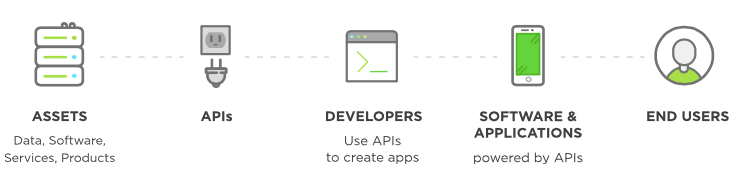
\includegraphics[scale=0.6]{API.png}
\caption{APIs }
\label{fig:fig1}
\end{figure}

That's the reason why KAOUN, a Tunisian FinTech start-up, decided to create its own developers API for its main product FLOUCI which is a mobile payment solution. This project will expand FLOUCI to the developers world and unleash the full potential of the product, also it could take FLOUCI into new markets and open doors for unlimited integrations.\newline


The following report is a synthesis of the efforts done to build FLOUCI developers API.

 To detail the process of our work, we have divided this report into XX chapters representing the different aspects of our project.

In the first chapter, entitled Project scope, we started with a presentation of the host company. Afterwards, we gave an overview of our project and we detailed the followed methodology for its realization.


The second chapter is about the development disciplines and rules we set during our project development life cycle. It's a detailed explanation of the development practices needed to start our project development in the most efficient way possible. 



We close our work with a general conclusion in which we try to evaluate our contribution as well as we develop our vision for the project's potential improvements.




\end{spacing}

\fancyhf{}
\fancyhead[R]{Introduction Generale}
\fancyfoot[R]{\thepage}
\renewcommand{\headrulewidth}{0.5pt}
\renewcommand{\footrulewidth}{0pt}



\setcounter{chapter}{0} %indique le numero reel du chapitre, pour la mini Table of Contents
\chapter{Project Scope}
\adjustmtc
\minitoc  %insert la minitoc

\graphicspath{{Chapter1/figures/}}
%==============================================================================
\pagestyle{fancy}
\fancyhf{}
\fancyhead[R]{\bfseries\rightmark}
\fancyfoot[R]{\thepage}
\renewcommand{\headrulewidth}{0.5pt}
\renewcommand{\footrulewidth}{0pt}
\renewcommand{\chaptermark}[1]{\markboth{\MakeUppercase{\chaptername~\thechapter. #1 }}{}}
\renewcommand{\sectionmark}[1]{\markright{\thechapter.\thesection~ #1}}

\begin{spacing}{1.2}
%==============================================================================

\section*{Introduction}
This chapter is dedicated to the presentation of our project's general scope.
This will include an introduction of the host company Kaoun and it's main product Flouci. Also, we will give an overview of the developer API project. After that, we will describe the chosen methodology that we followed during the realization of our project.
\section{Host company presentation}
In The first section of the report, we will introduce Kaoun, The host company that made the project possible.
\subsection{Presentation of Kaoun}
\begin{center}
	
\includegraphics[scale=0.2]{kaounlogo.png}
\end{center}



Kaoun is a new FinTech company that builds reliable infrastructure for payments and credits in Tunisia, and whose mission is to enable all individuals and businesses to access financial services using any phone, anywhere, anytime.

Kaoun's first product, Flouci, is a mobile and web payment application built on top of a unique decentralized inter and intrabank infrastructure that allows instant transactions for peer to peer transfers and merchant payments. Kaoun plans to work with governments, traditional banks, mobile operators, and microfinance institutions to fix the lag between technology adoption and financial inclusion by reducing the barriers to entry for the unbanked and the underbanked.








\subsection{Presentation of Flouci}
\begin{center}
	
\includegraphics[scale=0.2]{floucilogo.png}
\end{center}
Flouci is the first wallet designed to innovate mobile payment in Tunisia. It serves as a quick, easy, and convenient way to open a bank account, send and receive money, and pay different merchants in-person or online, all from within the app.
\begin{itemize}
  \item \textbf{Open an account:}

  In order to create a Flouci account, you either link your Flouci wallet to an existing bank account or follow the step-by-step KYC (Know Your Customer) guide to create an account with one of our partner financial institutions. Once you have your wallet and your QR code, you can start sending and receiving money and paying merchants using your phone.

  \item \textbf{Send and receive money:}

  Once you create a Flouci account, you can send and receive money to and from anybody that has a flouci account/wallet. It's easy, cheap, and secure. And the best part is that it's practically instant. All you have to do is enter their number or scan their personal QR code to access their profile. You then enter the amount and confirm. You both then receive a confirmation SMS and you're done.
  \item \textbf{Pay merchants:}

  Through Flouci, you have access to a wide range of partner merchants across Tunisia. You can pay through the app by just scanning the QR code shown on the counter of the merchant. No waiting lines, no more looking for change or realizing you forgot your wallet at home.
\end{itemize}

\section{Project overview}
In this section, we will start by presenting the developers API project context, then we will set our project goals.
\subsection{Project Context}
Flouci in its first version made it possible for users to pay merchants in simple steps and without the need of cash.
Flouci main app made it easy to transfer money between accounts. With the use of QR codes, users can send and receive money in less than 5 seconds.

\subsection{Flouci limitations}
The market is rapidly shifting toward online e-commerce sites with companies like Jumia, Tayara and many other introducing their solutions in Tunisia.

In its current implementation, Flouci is not able to integrate into any form of online payments due to the lack of its implementation.

Facing this problem and a fast moving e-commerce market the company had to move toward implementing a solution for developers.

The API should make it possible for developers to link their Flouci wallets to their e-commerce sites and add Flouci as an easy and instant payment method.
\subsection{Project goals}
To bring developers to the Flouci world and allow e-commerce owners to introduce a mobile payment solution Kaoun has decided to build its own developer API from scratch and provide an easy way to accept payments in few simple steps. This presented the opportunity for us to turn this problem into the main objective of our graduation project.

By the end of our project, we need to achieve these goals :
\begin{itemize}
  \item \textbf{Create Account:}
  Any developer should be able to create a Flouci developer account from the web platform, basic information is needed to open an account.

  Also, it should be possible to use an existing Flouci account and switch it to developer mode.
  \item \textbf{Create App and link Flouci wallet:}

  The web interface should offer the possibility to create an App and link it an existing wallet. A two steps verification system should be put in place to verify ownership of the wallet.
  To verify transaction developer could choose between two modes:
  \begin{itemize}
  \item \textbf{Active mode:} Activate an endpoint to verify transactions by id.
  \item \textbf{Passive mode:} Configure a webhook to receive transactions info once validated.
   \end{itemize}
   A unique token is generated for each app to allow client integration.
  \item \textbf{Integrate Flouci client:}

 Once the App is configured the developer can easily add Flouci as a payment method with the token provided.
  \item \textbf{Check App analytics:}

  Every App should enable a dashboard for the developer to monitor sales and check a set of KPI's.
\end{itemize}
\section{Methodology}

In this section, we will go through the importance of having a fixed methodology in a software development project, as well as our choice for this project and the reasons behind it.
\subsection{Agile methodology}
In every professional IT project, it is essential to adopt a methodology
of work in order to guarantee a good organization of tasks and to define the different phases
through which the project passes.
Since their appearance, agile \cite{agile}  development methods have considerably improved
the quality of the software and have reduced their production time. Thanks to its nature,
incremental and collaborative, such a methodology allows taking into account the evolution
of the customer's needs. Agile methodologies are based on four main values:
\begin{itemize}
	\item They promote interaction between the various parties involved in the project.
\item They replace exhaustive documentation with concrete functionalities.
\item The client participates in the project throughout its implementation instead of defining contracts
that formalize the relationship with the client.
\item It is necessary to accept the likely changes during the implementation process.
\end{itemize}

We chose the Kanban methodology for our project for three reasons:

\begin{itemize}
	\item Visually see work in progress.
	\item Empower teams to self-manage visual processes and workflows.
	\item Kanban boards can easily be managed on different free tools, like Trello, MeisterTask or GitKraken which we will be using in our project.
\end{itemize}



\subsection{Kanban methodology}

In general, Kanban\cite{kanban} is a scheduling system for lean and other JIT processes. In a Kanban process, there are physical (or virtual) "cards" called Kanban that move through the process from start to finish. The aim is to keep a constant flow of Kanban so that as inventory is required at the end of the process, just that much is created at the start.


When used for software development, Kanban uses the stages in the software development lifecycle (SDLC) to represent the different stages in the manufacturing process. The aim is to control and manage the flow of features (represented by Kanban cards) so that the number of features entering the process matches those being completed.

Kanban is an agile methodology that is not necessarily iterative. Processes like Scrum have short iterations which mimic a project lifecycle on a small scale, having a distinct beginning and end for each iteration. Kanban allows the software be developed in one large development cycle. Despite this, Kanban is an example of an agile methodology because it fulfills all twelve of the principles behind the Agile manifesto, because whilst it is not iterative, it is incremental.

The principle behind Kanban that allows it to be incremental and Agile, is limited throughput. With no iterations a Kanban project has no defined start or end points for individual work items; each can start and end independently from one another, and work items have no pre-determined duration for that matter. Instead, each phase of the lifecycle is recognized as having a limited capacity for work at any one time. A small work item is created from the prioritized and unstated requirements list and then begins the development process, usually with some requirements elaboration. A work item is not allowed to move on to the next phase until some capacity opens up ahead. By controlling the number of tasks active at any one time, developers still approach the overall project incrementally which gives the opportunity for Agile principles to be applied.

Kanban projects have Work In Progress (WIP) limits which are the measure of capacity that keeps the development team focused on only a small amount of work at one time. It is only as tasks are completed that new tasks are pulled into the cycle. WIP limits should be fine-tuned based on comparisons of expected versus actual effort for tasks that complete.

Kanban does not impose any role definition as say, Scrum does and along with the absence of formal iterations, role flexibility makes Kanban attractive to those who have been using waterfall-style development models and want to change but are afraid of the initial upheaval something like Scrum can cause while being adopted by a development team.

\subsection{Lean software development}

Lean Software Development \cite{lean} is a set of principles to deliver software according to the principles of lean manufacturing. In a lean environment, activities or processes that result in the expenditure of effort and/or resources towards goals that are not producing value for the customer should be eliminated. Essentially, lean is centered on preserving value with less work. Lean approaches are often called six-sigma or Just-In Time (JIT).

\subsection{Project orientations}
After a deep study of existing methodologies, we decided to divide our project into three sprints.
we will dedicate the first sprint to the initial project set up including the DevOps, in the second sprint we will be implementing the developer platform and finally, we will implement the checkout module in the last sprint.

In each sprint, we will have a Kanban board to divide the sprint into incremental tickets.

\subsection{Project Backlog}
the backlog is intended to collect all the customer's needs that the project team must realize. Therefore it contains the list of functionalities involved in the creation of the product, as well as all the elements requiring the intervention of the project team. All the elements included in the backlog are classified by priority indicating the order of their realization.
\newpage




\begin{table}[!h]
\centering
\caption{Use case description table}
\begin{tabularx}{\linewidth}{|c|X|c|c|}
\hline
ID & \multicolumn{1}{c|}{User Story} & Estimation & Priority \\ \hline
1 & As an unauthorized user i want to create a new account. &  3 & 1  \\  \hline
2 & As an unauthorized user i want to recover my account using my email. &  1 & 3 \\ \hline
3 & As an unauthorized user i want to read the documentation. & 2 & 2 \\ \hline
4 & As an unauthorized user i want to login in to my account. & 3 & 1 \\ \hline
5 & As an authorized user i want to logout in to my account. & 1 & 1 \\ \hline
6 & As an authorized user i want to create an integration app. & 3 & 1 \\ \hline
7 & As an authorized user i want to  enable/disable my integration app. & 1 & 3 \\ \hline
8 & As an authorized user i want to  revoke my integration app. & 1 & 2 \\ \hline
9 & As an authorized user i want to  generate my integration app credentials. & 1 & 1 \\ \hline
10 & As an authorized user i want to check my integration app orders. & 2 & 2 \\ \hline
11 & As an authorized user i want to check my integration app transaction number. & 1 & 3 \\ \hline
12 & As an authorized user i want to check my integration app gross sales. & 1 & 2 \\ \hline
13 & As an authorized user i want to change my account settings. & 2 & 3 \\ \hline
14 & As an authorized user i want to integrate Flouci button in my website using my integration app public token. & 3 & 1 \\ \hline
15 & As an authorized user i want to accept payments in my website using my integration app private token. & 3 & 1 \\ \hline
16 & As an authorized user i want to reimburse payments orders. & 3 & 2 \\ \hline
\end{tabularx}
\end{table}

\section*{Conclusion}

This first chapter allowed us to define the general boundaries of our project.

We gave an introduction of our host company and the motivations behind the project.
We studied the project context and the existing similar projects, we took a look into the three biggest implementations.

In The end we set the basis of the project by fixing a methodology to follow in the development and realization of the project.





%==============================================================================
\end{spacing}


\setcounter{chapter}{1}
\chapter{Requirements analysis and specification}
\minitoc %insert la minitoc
\graphicspath{{Chapter2/figures/}}

%\DoPToC

%==============================================================================
\pagestyle{fancy}
\fancyhf{}
\fancyhead[R]{\bfseries\rightmark}
\fancyfoot[R]{\thepage}
\renewcommand{\headrulewidth}{0.5pt}
\renewcommand{\footrulewidth}{0pt}
\renewcommand{\chaptermark}[1]{\markboth{\MakeUppercase{\chaptername~\thechapter. #1 }}{}}
\renewcommand{\sectionmark}[1]{\markright{\thechapter.\thesection~ #1}}

\begin{spacing}{1.2}
%==============================================================================
\section*{Introduction}
In this chapter we will begin our project by a study of the existing checkout developers API's on the market, then we will start the requirements analysis to identify the different actors that will interact with our system, as well as the features required in our project.
\section{Study of the existing}
In The world of e-commerce, a lot of payments methods exists.  Most of the methods are credit card related and offer the possibility to pay using the card number and the three digits code.

In our case, Flouci offer payments through QR codes scans. Although the payment steps on the user side are different, the developer API should offer similar functionalities.


Below is a list of world leader online payment API's:
\begin{itemize}
  \item \textbf{Stripe:}

 The Stripe API is organized around REST. The API has predictable resource-oriented URLs, accepts form-encoded request bodies, returns JSON-encoded responses, and uses standard HTTP response codes, authentication, and verbs.

You can use the Stripe API in test mode, which does not affect your live data or interact with the banking networks. The API key you use to authenticate the request determines whether the request is live mode or test mode.

\begin{figure}[!ht]\centering
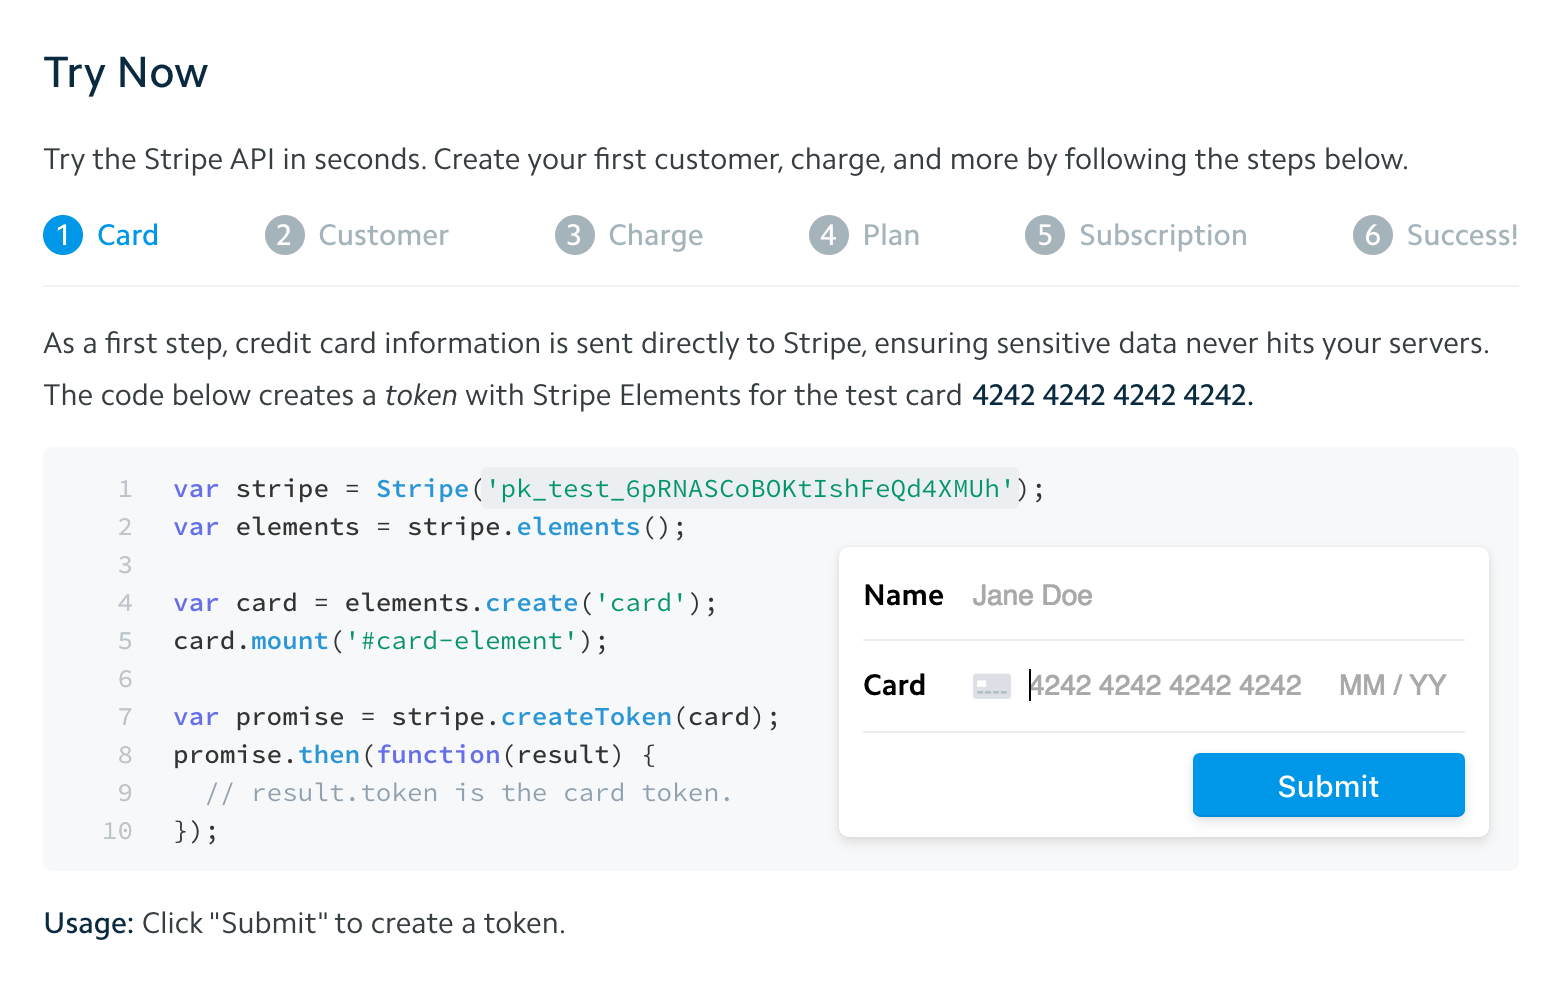
\includegraphics[scale=0.3]{stripe.png}
\caption{Stripe Api}
\label{fig:fig1}
\end{figure}

  \item \textbf{Paypal:}

  The PayPal APIs are HTTP-based RESTful APIs that use OAuth 2.0 for authorization. API request and response bodies are formatted in JSON.

\begin{figure}[!ht]\centering
\includegraphics[scale=0.3]{PayPal.png}
\caption{PayPal Api}
\label{fig:fig1}
\end{figure}
\newpage
\item \textbf{Twint:}

Twint is the closest implementation to Flouci, it offers payments through QR code scans.

The plugin allows QR code generation on the web page, it also creates a code for each transaction, It serves to confirm payments.
\begin{figure}[!ht]\centering
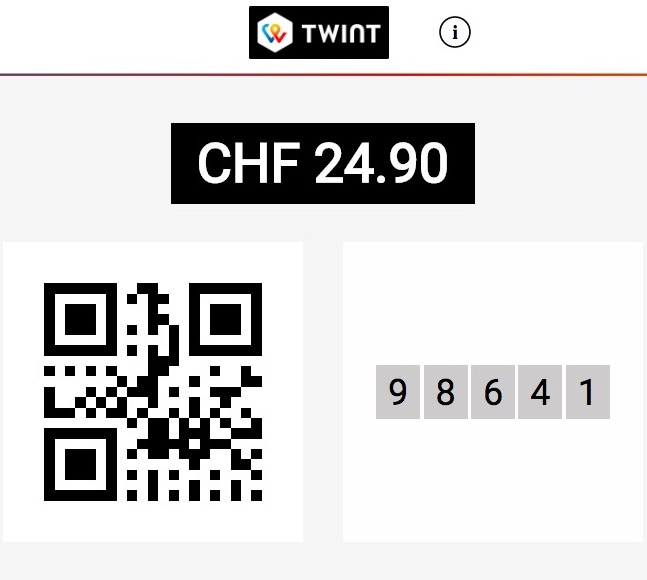
\includegraphics[scale=0.3]{twint.jpg}
\caption{Twint Pop-up}
\label{fig:fig1}
\end{figure}
  \end{itemize}
  
  

\section{Requirements specification}
A good in-depth requirements specification is the key to a solid foundation of any project.
The motivation behind this section is to take a global look at the project and be able to understand all the requirements needed to achieve our goals.
\subsection{Actors identification}
Actors are any entity that plays a role in our system. They can be users or systems that interact with our system. We were able to identify the external and internal actors of our platform. 
\newline
Among the internal actors we find:
\begin{itemize}
  \item \textbf{Anonymous Developer:} He can navigate on all the public pages of the site which are
accessible without authentication including the documentation part. Also, he can register a developer account.
  \item \textbf{Registred Developer:} He can manage his account, create and manage app's and integrate them on e-commerce websites.
  \item \textbf{Flouci User:}  He can use the checkout API the pay online merchants.
\end{itemize}
The external actors who are necessary for our platform are:
\begin{itemize}
  \item \textbf{Wallets API:} Is needed to activate any app. The app should be linked to a Flouci wallet.
  \item \textbf{Payments API:} Is needed for online payments.
\end{itemize}
\subsection{Functional requirements}
In this section, we will understand the functional requirements of our project by studying the global use case of our system.
	\newline In the Figure \ref{fig:usecasediagram}, we showcase the \textbf{general use case diagram} and then with the Table \ref{tab:usecasediagram} we explain more in-depth the different use cases.
\begin{figure}[H]\centering
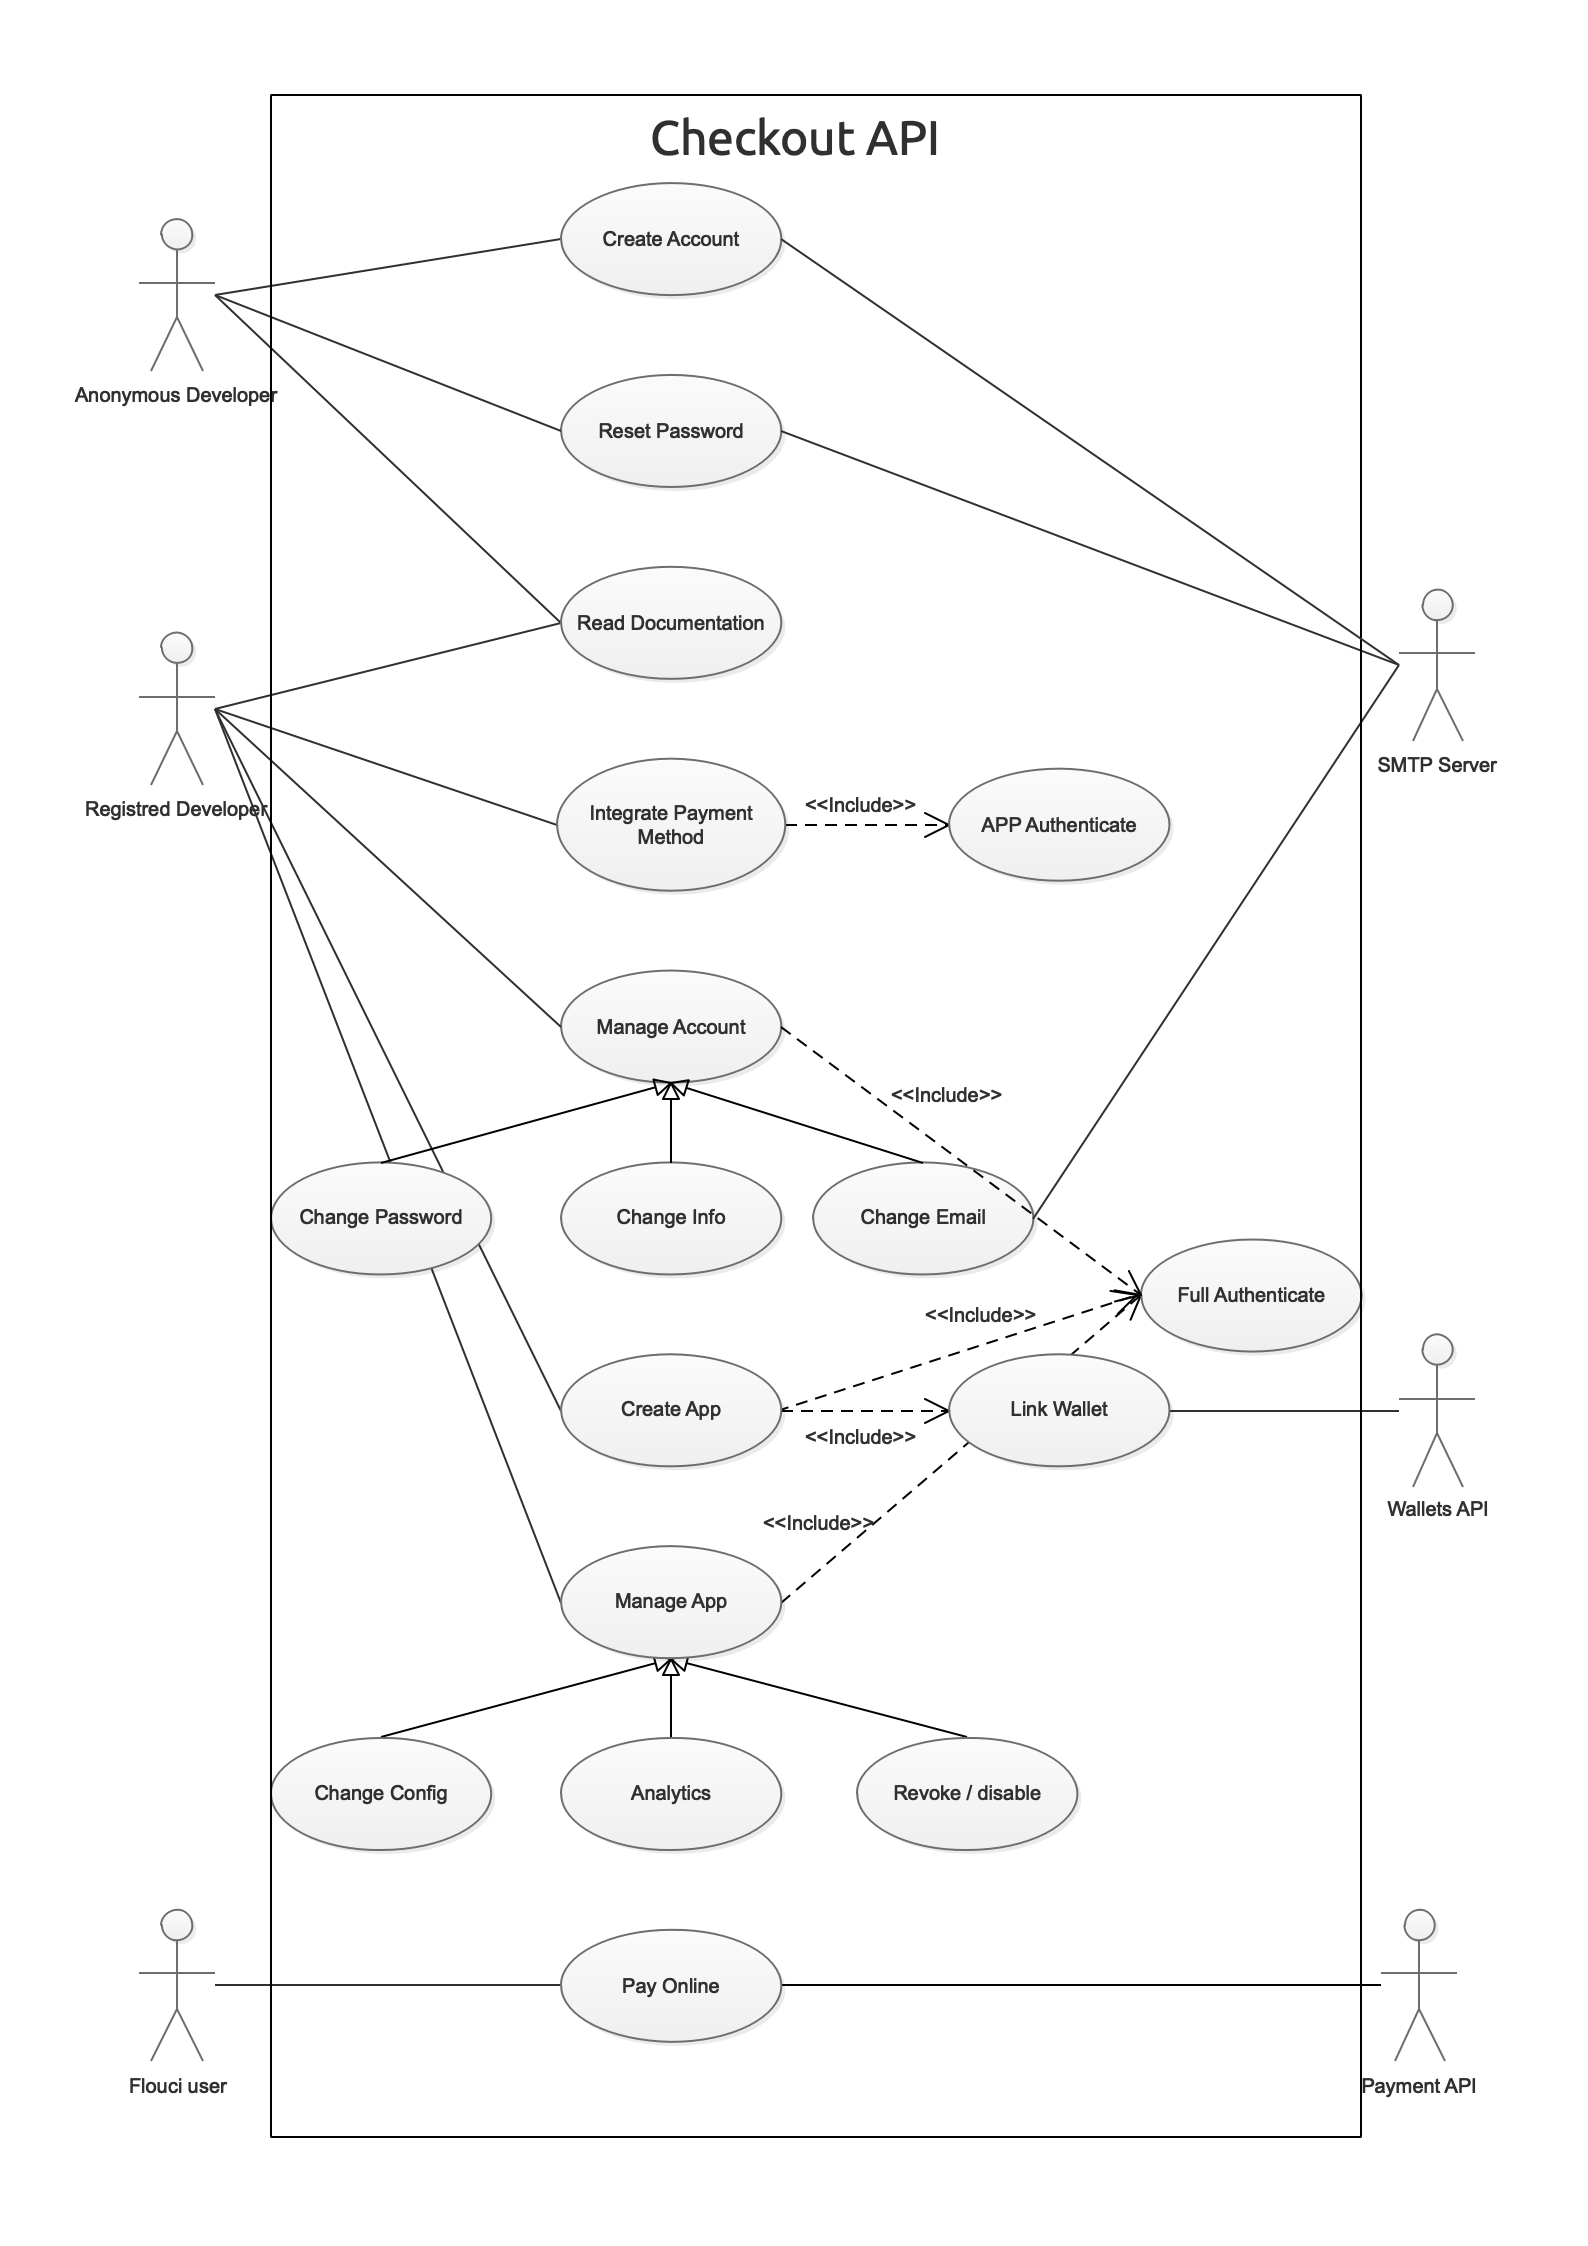
\includegraphics[scale=0.6]{GeneralUseCase.png}
\caption{General Use Case Diagram}
\label{fig:usecasediagram}
\end{figure}

\begin{table}[!h]
	\centering
	\caption{Use case description table}
	\footnotesize
	\begin{tabularx}
	{\linewidth}{|>{\centering{}\vspace*{\fill}}X|>{\centering{}\vspace*{\fill}}X|>{\vspace*{\fill}}X<{\centering{}}|}	
			\hline 
			 \bfseries Internal actor & \bfseries Use case &\bfseries External actor \\
			\hline 
			\multirow{3}{*}{Anonymous Developer}			&	Create Account: Any person with an email account can register for a Flouci developer account. 	&	SMTP Server			\\
			\cline{2-3}
				& Reset Password: In case a registered user forgets his password, he can reset it using his email address. 		&		SMTP Server		\\
				\cline{2-3}
					&	Read Documentation: Any person with access to the developer's platform can access the documentation.	&				\\
			\hline 
			\multirow{5}{*}{Registred Developer}					&	Read Documentation: The developer can access the documentation 	&				\\
			\cline{2-3}
			&	Integrate Payment Method: Any active app could be integrated into a commerce website and the integration only requires the public and private app tokens (App Authentication).	&				\\
			\cline{2-3}
					&	Manage Account:    The developer can change manage his account by changing his password, email or his basic info.	&		SMTP Server	\\
					\cline{2-3}
					&	Create App: An Authenticated developer can create an app and link it to a wallet with OTP verification through the Wallets API.	&			Wallets API	\\
					\cline{2-3}
					&	Manage App:	 An Authenticated  developer can check the analytics of his apps as well as tweak any app settings. &				\\		
					
			\hline 
			Flouci User	& Pay Online : With the pay with Flouci button on e-commerce websites, the Flouci user can quickly pay online merchants.  	&	Payment API	\\
			
			\hline
	\end{tabularx}
	\label{tab:usecasediagram}
\end{table}


\subsection{Non-functional requirements}
\subsubsection{Security}
When it comes to payment solutions security is the number one requirement to keep in mind.
Our solution implements many layers of security including: 
\begin{itemize}
	\item \textbf{HTTPS:} The platform only works on https mode, we use "Kaoun" trusted certificate.
	\item \textbf{JWT Token\cite{JWT}:}  Access to the platform is secured with JWT tokens, managing apps is only possible with this token.
	\item \textbf{Private / Public Tokens for Apps:}  In order to accept Payments Flouci user sign payments attached to the app public key and the developer can only accept them if he has the private key.
	App public keys can be revoked.
\end{itemize}
\subsubsection{Documentation}
An API is only usable with proper documentation, So in order to get developers to implement our solutions, we should have easy and understandable documentation. The documentation is accessible in our platform.\subsubsection{Logging}
Our Solution is using "logstash" to forward logs to our ELK\cite{ELK} stack, different log levels are used and we implemented a lot of metrics and dashboards on our kibana.

\begin{figure}[H]\centering
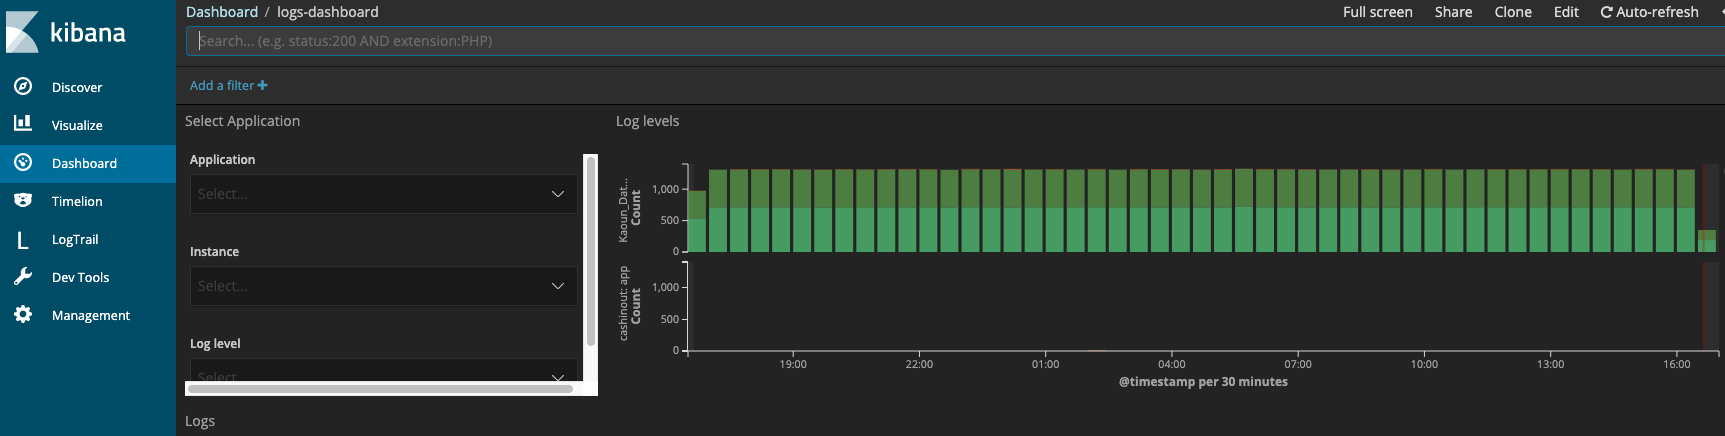
\includegraphics[scale=0.3]{ELK.png}
\caption{Kibana Dashboard}
\label{fig:usecasediagram}
\end{figure}

\subsubsection{Integrability}
Flouci online payment method can be easily integrated into any e-commerce website. It only requires an HTML form in the front end and an API call to accept payments on the backend.

\subsubsection{Extensibility}
Our payment method should allow extensibility and add more payment method other than the QR code scans. 
\subsubsection{Legal}
On the legal side, we should be compliant with the Tunisian laws and only enable appropriate users to accept payments.
This is achieved on the app creation level, at the stage of linking the wallet.
\subsubsection{Privacy}
Flouci users privacy should be considered at the highest levels, payment history and activities should be seen only by the persons with the right permissions.
\subsubsection{Ergonomics}
To guarantee a good control of our project and to simplify the interaction with the final users, we support our analysis of functional needs with mock-ups that model the different interfaces of our final product. These models are made by the "Adobe XD" tool and they are compliant with the overall Kaoun prouducts user experience. \newline Figure \ref{checkoutScreen} represents the checkout pop-up on e-commerce websites.
\newline Figure \ref{developersPlatform} represents the Developers API platform.

\begin{figure}[H]\centering
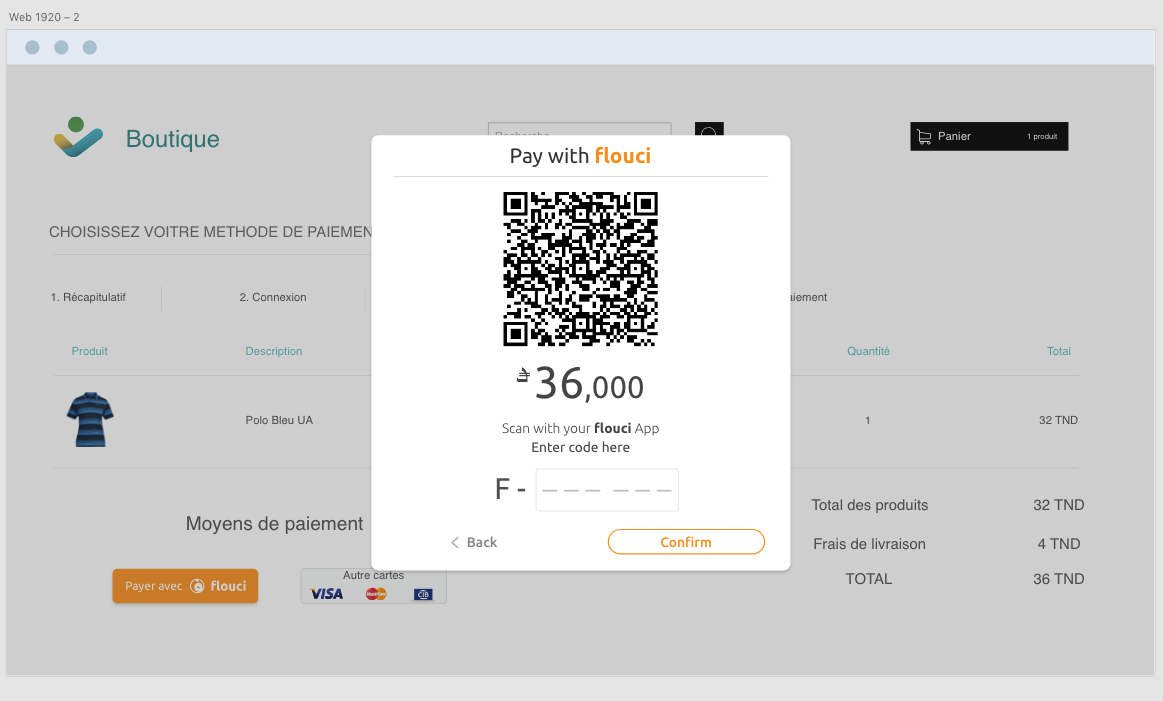
\includegraphics[scale=0.4]{Checkout_screen}
\caption{Checkout pop-up mock-up}
\label{checkoutScreen}
\end{figure}

\begin{figure}[H]\centering
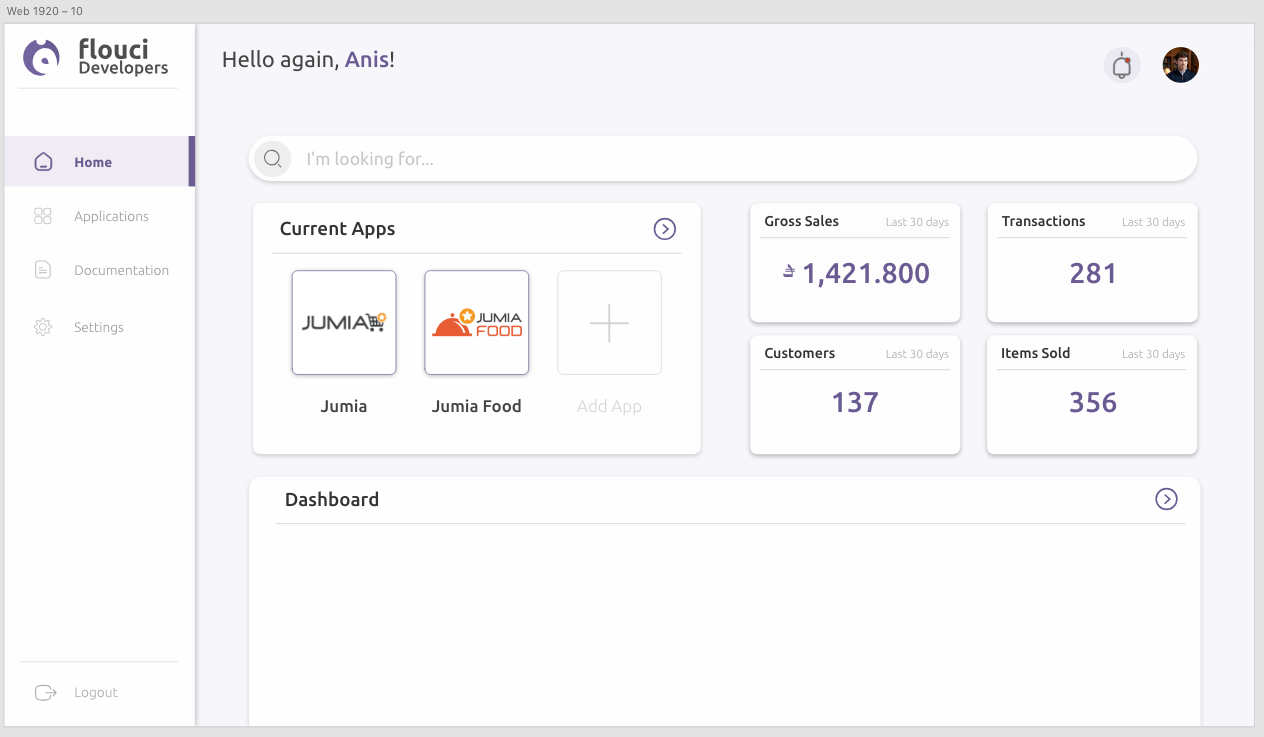
\includegraphics[scale=0.4]{web_screen}
\caption{Developers platform mock-up}
\label{developersPlatform}
\end{figure}

\section*{Conclusion}
In this chapter, we took the time to think about different aspects of our project, we went through detailed analysis in order to comprehend the project boundaries. After this we can launch our project development cycles which what we will be the topic of our next chapter.
%==============================================================================
\end{spacing}


\setcounter{chapter}{2}
\chapter{Sprint 1: Project Launch}
\minitoc %insert la minitoc
\graphicspath{{Chapter3/figures/}}

%\DoPToC
%==============================================================================
\pagestyle{fancy}
\fancyhf{}
\fancyhead[R]{\bfseries\rightmark}
\fancyfoot[R]{\thepage}
\renewcommand{\headrulewidth}{0.5pt}
\renewcommand{\footrulewidth}{0pt}
\renewcommand{\chaptermark}[1]{\markboth{\MakeUppercase{\chaptername~\thechapter. #1 }}{}}
\renewcommand{\sectionmark}[1]{\markright{\thechapter.\thesection~ #1}}

\begin{spacing}{1.2}

%==============================================================================

\section*{Introduction}
This chapter is introducing the software development disciplines and rules followed during the achievement of our project. In order to have a clear development structure, a development process must be set in place in the earliest stage of our project life.

Our development process is a combination of different practices like Test-driven development and DevOps.

\section{Kanban Tickets Life Cycle}
Following the Kanban methodology, our project is decomposed to small tickets with limited scopes. The tickets are developed in an incremental way following priority order, and together they shape our project to its final version.
The figure \ref{fig:kanban} shows our product board.
\begin{figure}[H]\centering
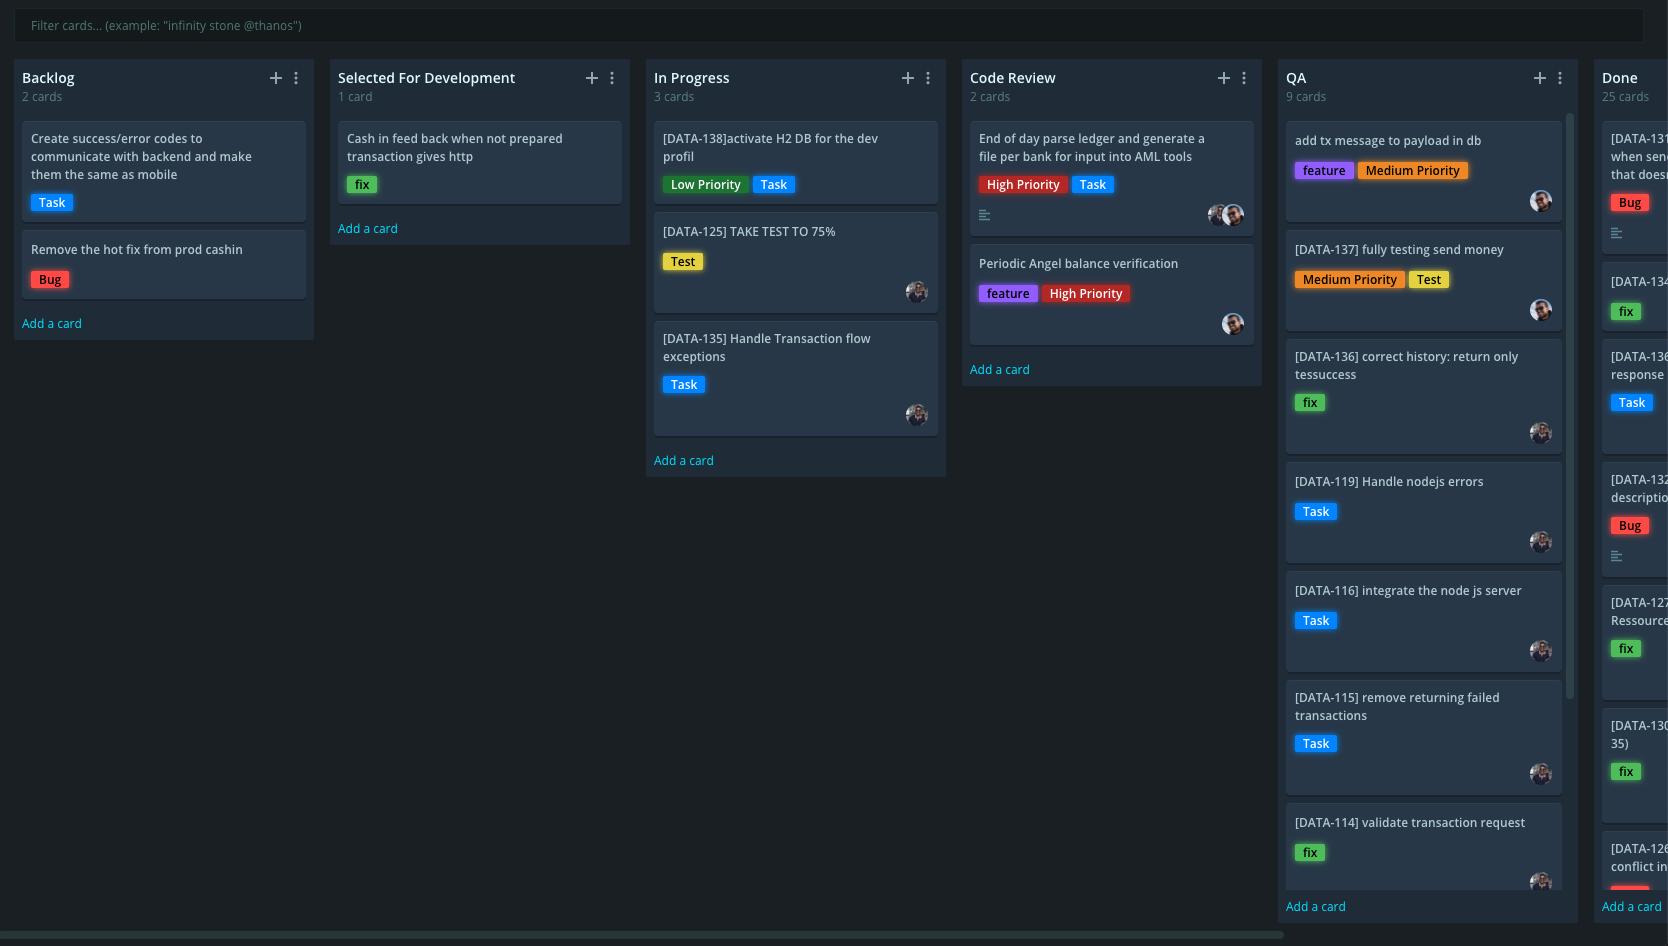
\includegraphics[scale=0.3]{kanban_board.png}
\caption{Kanban Board}
\label{fig:kanban}
\end{figure}
\subsection{Backlog}
All tickets are created in the "Backlog" stage, any work that needs to be done is formed into a ticket.


The ticket needs to have a self-explanatory description, to make it simple for the developer to start working on it without the need for further explanation.

A Tag must be assigned to the ticket as well, tags could be referring to the nature of the work to do (e.g. Bug, Fix, Task), or the scope e.g. Back-end, Front-end, DevOps.

In the end, the ticket priority must be set following a priority system set by the development team. The system could relay on numerical values (e.g. 0 having the least priority, 1, 2), or having specific tags (e.g. LOW, MEDIUM, HIGHT, URGENT) which we will be using in our project.

Tickets could only move from "Backlog" to "Selected For Development".
\subsection{Selected For Development}
In the "Selected For Development" stage developers have access to the tickets. They have to tackle the ticket following the priority system and the tag matching their expertise (Back-end, Front-end).

Once they choose a ticket they must assign it to their name, move it to the "In Progress" stage and create a git branch with the ticket name and finally start developing.

Tickets could only move from "Selected For Development" to "In Progress".
\subsection{In Progress}
The "In Progress" stage serves as a safety mechanism to avoid having two developers working on the same ticket.

This stage indicates that the tickets are taking care of, it also shows the person developing the ticket.

If the developer finishes his work he should move the ticket to "Code Review" stage and make a pull request of the branch.


In the case of failure, the ticket should go back to the "Selected For Development" stage.
\subsection{Code Review}
Once a ticket is in the "Code Review" stage, the project manager should open the pull request and check the code committed by the developer.

In case of approval, the pull request is merged and deployed, the ticket then is moved to "QA".


In case of disapproval, the project manager leaves comments on the pull request and moves the ticket back to "In progress". The developer then needs to check the code and fix the issue.
\subsection{QA}
In the "QA" stage tickets are tested by fellow developers, the functionality of the ticket should be tested on an environment similar to the production environment, also developer should push the test to the limit and test all edge cases.

If all developers approve that the code is working fine in every possible scenario the ticket is moved to do, otherwise, the ticket info should be updated with the issues encountered and the ticket is moved back to the "In Progress" stage.

\subsection{Done}
All tickets should finally be moved to the "Done" stage, this stage groups all the work is done and keeps track of the progress of the development.


After a fixed time tickets get archived to gain space in the Kanban board.

\section{Gitflow workflow }
Gitflow Workflow is a Git workflow design that was first published and made popular by Vincent Driessen at nvie. The Gitflow Workflow defines a strict branching model designed around the project release. This provides a robust framework for managing larger projects.

Gitflow is really just an abstract idea of a Git workflow. This means it dictates what kind of branches to set up and how to merge them together. 
The figure \ref{fig:git} shows our different branches and our merging strategy.

\begin{figure}[!ht]\centering
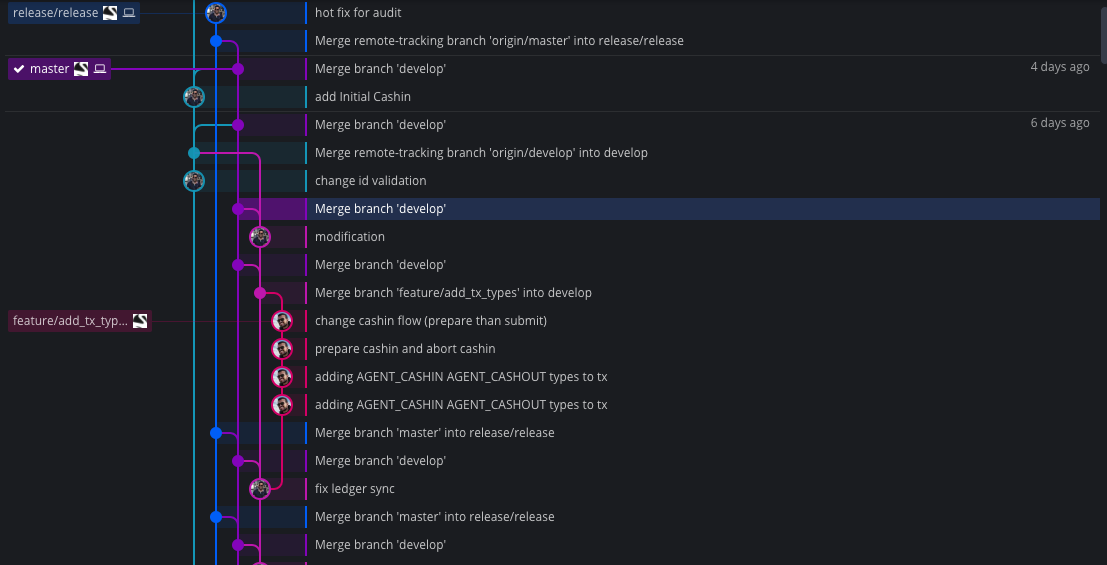
\includegraphics[scale=0.4]{git_workflow.png}
\caption{Git Workflow}
\label{fig:git}
\end{figure}

\newpage
\subsection{Feature Branch}
The feature branch is created by the developer for every Kanban ticket he tackles. When moving the ticket to the "In Progress" stage the branch should be created with the same name as the ticket.

All the development specific to the scope of the ticket should be done in the same branch, and in the end, the developer should make a pull request on the Develop Branch.
\subsection{Develop Branch}
The Develop branch presents the edge version of the product, it contains all newly developed features. This branch is the main branch to the internal project team, All newly developed feature is tested by developers on this branch, it maps to the "dev environment".

This branch could present a number of bugs because by nature it's a testing and validation branch of the latest developed code.

This branch is daily updated.
\subsection{Master Branch}
After tickets validation and bug fixes, the internal team merges a stable version of the product (Develop branch) to the Master branch. This branch maps to the staging environment and serves for testing on the company level.

All company projects depending on our project always use its staging version. The testing and integration with other projects should be verified extensively before merging to the production environment.

\subsection{Release Branch}
This is the production branch, code on this branch has been tested twice in both the dev and staging environments.

The branch is updated according to the release dates, it's the result of merging a stable master branch.

The branch maps to the prod environment and it's the actual branch used by the end user.
\subsection{Hotfix Branch}
As it is impossible to have a bug free software, we should take in consideration bugs popping in the prod environment.

Every bug discovered on the prod environment opens an urgent fix ticket, the ticket branch is based on the release branch and it's merged directly to the release branch after the fix.

This is a measure to quickly fix issues that have effects on the end user.




\section{Test-driven development}
"Test Driven Development"\cite{TDD} is a development technique that requires the writing of tests even before writing the first line of code.

In theory, the method requires the intervention of at least two different people, one person writes the tests, the other writes the code. This avoids problems related to subjectivity.

In practice things are more complicated, sometimes you develop alone or you write the tests yourself that guarantee the integrity of new functionality in a collaborative project.

The TDD can be divided into 5 distinct steps as shown in the figure  \ref{fig:tdd}:
\begin{enumerate}
	\item  Write a test.
	\item Check that it fails.
	\item Write the code enough for the test to pass.
	\item Check that the test passes.
	\item Optimize the code and check that there is no regression.
\end{enumerate}

\begin{figure}[!ht]\centering
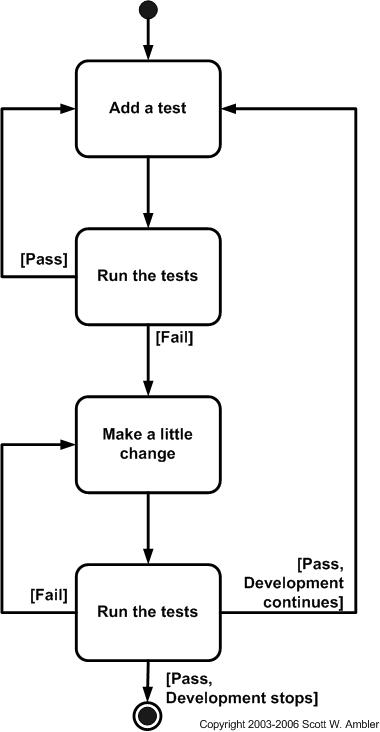
\includegraphics[scale=0.6]{tddSteps.jpg}
\caption{TDD Steps}
\label{fig:tdd}
\end{figure}
\newpage
In our project, The development of every ticket starts by writing the test. A pull request can only be approved if it contains and passes the new test.

This discipline enables our project to benefits from the DevOps world, As it's important to have a test for the CI-CD process to be defined.


\section{DevOps}
DevOps\cite{devops} is a set of practices that automates the processes between software development and IT teams, in order that they can build, test, and release software faster and more reliably.

In our project we need to have an autonomous testing and deployment process to maintain our three environments:
\begin{itemize}
	\item \textbf{Dev environment:} Represents the Develop branch and used for internal team testing.
	\item \textbf{Staging environment:} Represents the Master branch and used for a company level testing.
    \item \textbf{Prod environment:} Represents the Release branch and used by the end user.
\end{itemize}

With every branch push our CI-CD server (Jenkins) triggers an automatic script that consists of a set of predefined steps.

The steps behave slightly different according to the branch name. 
Our pipeline is shown in the figure \ref{fig:jenkins}
\begin{figure}[!h]\centering
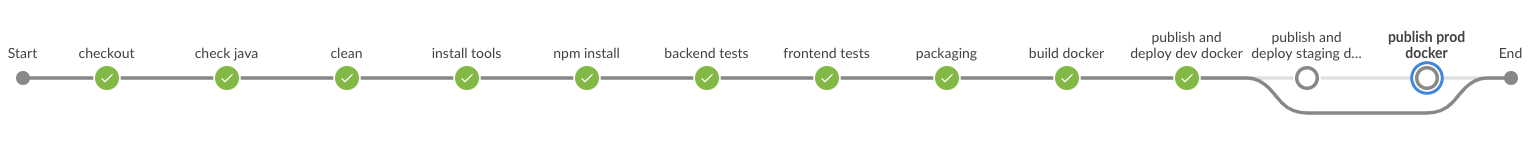
\includegraphics[scale=0.3]{jenkins.png}
\caption{Kaoun logo�}
\label{fig:jenkins}
\end{figure}
\subsubsection{Preparation}
The first step, of every build is getting the branch code and preparing a clean environment containing all the dependencies required to run our project.
\subsubsection{Testing}
In this step, all tests are executed for both backend and frontend. A full report is created with the test results.
We can only continue the build if all tests are passed gracefully otherwise the job is terminated.
\subsubsection{Quality Measurements}
In this step, the code is inspected by the open-source platform SonarQube.

The step performs automatic reviews with static analysis of code to detect bugs, code smells, and security vulnerabilities.
\subsubsection{Dockerization}
If all testing and quality measures are approved we proceed to the Dockerization of our project.
This step creates a standard artifact that can be deployed on any infrastructure without the need for specific configurations for different servers.

If the Docker images are created successfully, it will be tagged latest and pushed to the Docker Hub.

\subsubsection{Deployment}
In the last step of the build, and according to the branch name the new artifact is deployed to the convenient server (dev, staging, prod).

On every target server, we have a docker swarm cluster to deploy the new version of the product.
The swarm cluster is also configured with the different environment variables as secrets to protect the different credentials (database, cloud services\dots).
\section{Tools}
In the section, we will present the set of tools that make it possible to follow the development disciplines mentioned above. The tools also help the automation of the processes.
\subsection{AdobeXD}
"Adobe XD"\cite{AdobeXD} is a vector-based tool developed and published by Adobe Inc for designing and prototyping user experience for web and mobile apps.
\subsection{Bitbucket}
"Bitbucket"\cite{Bitbucket} is a web-based version control repository hosting service owned by Atlassian, for source code and development projects that use Git revision control systems.
\subsection{GitKraken Glo Boards}
"GitKraken Glo Boards" is a software that manage boards and tickets. In our case the Kanban board is created and managed on GitKraken.
\subsection{Docker}
"Docker"\cite{Docker} is a tool designed to make it easier to create, deploy, and run applications by using containers. Containers allow a developer to package up an application with all of the parts it needs, such as libraries and other dependencies, and ship it all out as one package. By doing so, thanks to the container, the developer can rest assured that the application will run on any other machine regardless of any customized settings that machine might have that could differ from the machine used for writing and testing the code.
\subsection{Docker Swarm}
As a platform, Docker has revolutionized the manner software was packaged. "Docker Swarm" \cite{Dockerswarm} or simply Swarm is an open-source container orchestration platform and is the native clustering engine for and by Docker. Any software, services, or tools that run with Docker containers run equally well in Swarm. Also, Swarm utilizes the same command line from Docker.

Swarm turns a pool of Docker hosts into a virtual, single host. Swarm is especially useful for people who are trying to get comfortable with an orchestrated environment or who need to adhere to a simple deployment technique but also have more just one cloud environment or one particular platform to run this on.
\subsection{Jenkins}
In order to have our CI/CD environment, we used "Jenkins" \cite{Jenkins} which is an open source automation server that helps you to automate the non-human part of the software development process.

"Jenkins" is a stand-alone open source automation server that can be used to automate all kinds of tasks related to software creation, testing, delivery or deployment.
\subsection{SonarQube}
"SonarQube"\cite{SonarQube} (formerly Sonar) is an open-source platform developed by SonarSource for continuous inspection of code quality to perform automatic reviews with static analysis of code to detect bugs, code smells, and security vulnerabilities on 20+ programming languages.

"SonarQube" offers reports on duplicated code, coding standards, unit tests, code coverage, code complexity, comments, bugs, and security vulnerabilities.

\section*{Conclusion}
We went through the Kanban methodology in practice, explaining the different steps of the incremental code writing.

 We also set the rules of the git branching model we will be using in our development process, as well as the test-driven development discipline to follow for every branch.

We tackled our DevOps setup and the different steps of the automation process from code writing to project deployment.

In the end, we presented the tools we will be using in our project development life cycle.

In the next chapter will start our first sprint entitled "Project Launch". The sprint is about setting up the right development disciplines and practices.


%==============================================================================
\end{spacing}


\setcounter{chapter}{3}
\chapter{Sprint 2: User and App Managment}
\minitoc %insert la minitoc
\graphicspath{{Chapter4/figures/}}

%\DoPToC
%==============================================================================
\pagestyle{fancy}
\fancyhf{}
\fancyhead[R]{\bfseries\rightmark}
\fancyfoot[R]{\thepage}
\renewcommand{\headrulewidth}{0.5pt}
\renewcommand{\footrulewidth}{0pt}
\renewcommand{\chaptermark}[1]{\markboth{\MakeUppercase{\chaptername~\thechapter. #1 }}{}}
\renewcommand{\sectionmark}[1]{\markright{\thechapter.\thesection~ #1}}

\begin{spacing}{1.2}

%==============================================================================
\section*{Introduction}
In order to integrate Flouci as a web payment method, we opted for an app model. This model consists of creating an app for each integration the developer wants to have, the app contains basic information about the e-commerce website and it's also linked to a Flouci account to accept payment directly.
\newline
In this chapter, we will start our project development. We will focus on implementing two linked parts of our application which are the user and app. 

\section{Flux Design Pattern}
Our solution is implemented with two main frameworks, Spring Boot and React JS.
Our back-end is entirely written with spring boot and serves as an api for our front-end developed with react.

Using React Js we had to follow a newly created design pattern called Flux. The pattern was created by Facebook and they define it as follow : 


\say{Flux\cite{Flux} is the application architecture that Facebook uses for building client-side web applications. It complements React's composable view components by utilizing a unidirectional data flow. It's more of a pattern rather than a formal framework, and you can start using Flux immediately without a lot of new code.}

\begin{figure}[H]\centering
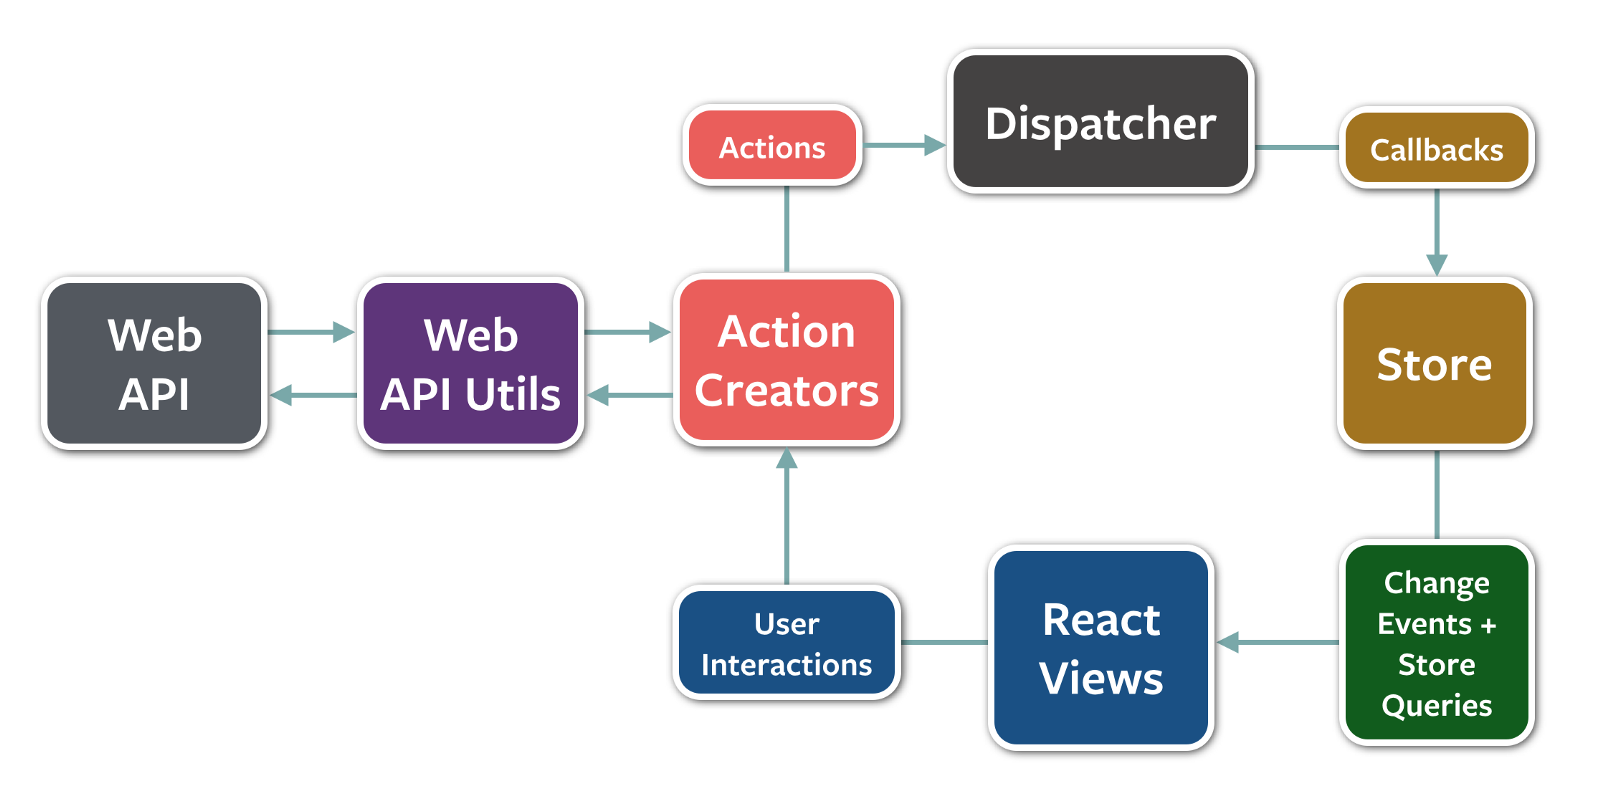
\includegraphics[scale=0.3]{Fluxdesignpattern.png}
\caption{Flux design pattern}
\label{usermanagementusecase}
\end{figure}

Flux is made up of 4 key elements:

\begin{itemize}
	\item \textbf{Actions:} Objects with property and data.
	\item \textbf{Stores:} Contain the application's state and logic.
	\item \textbf{The Dispatcher:} Processes registered actions and callbacks.
	\item \textbf{Views:} Listen to changes from the stores and re-render themselves.
\end{itemize}

\section{Sprint Use cases}
In this section, we will start by understanding the sprint specification by looking into the use cases diagrams.

\subsection{User management use case}
Each project starts with the user management section. This section is about the basic user management features.

The figure \ref{usermanagementusecase} shows the user management use case diagram.
\begin{figure}[H]\centering
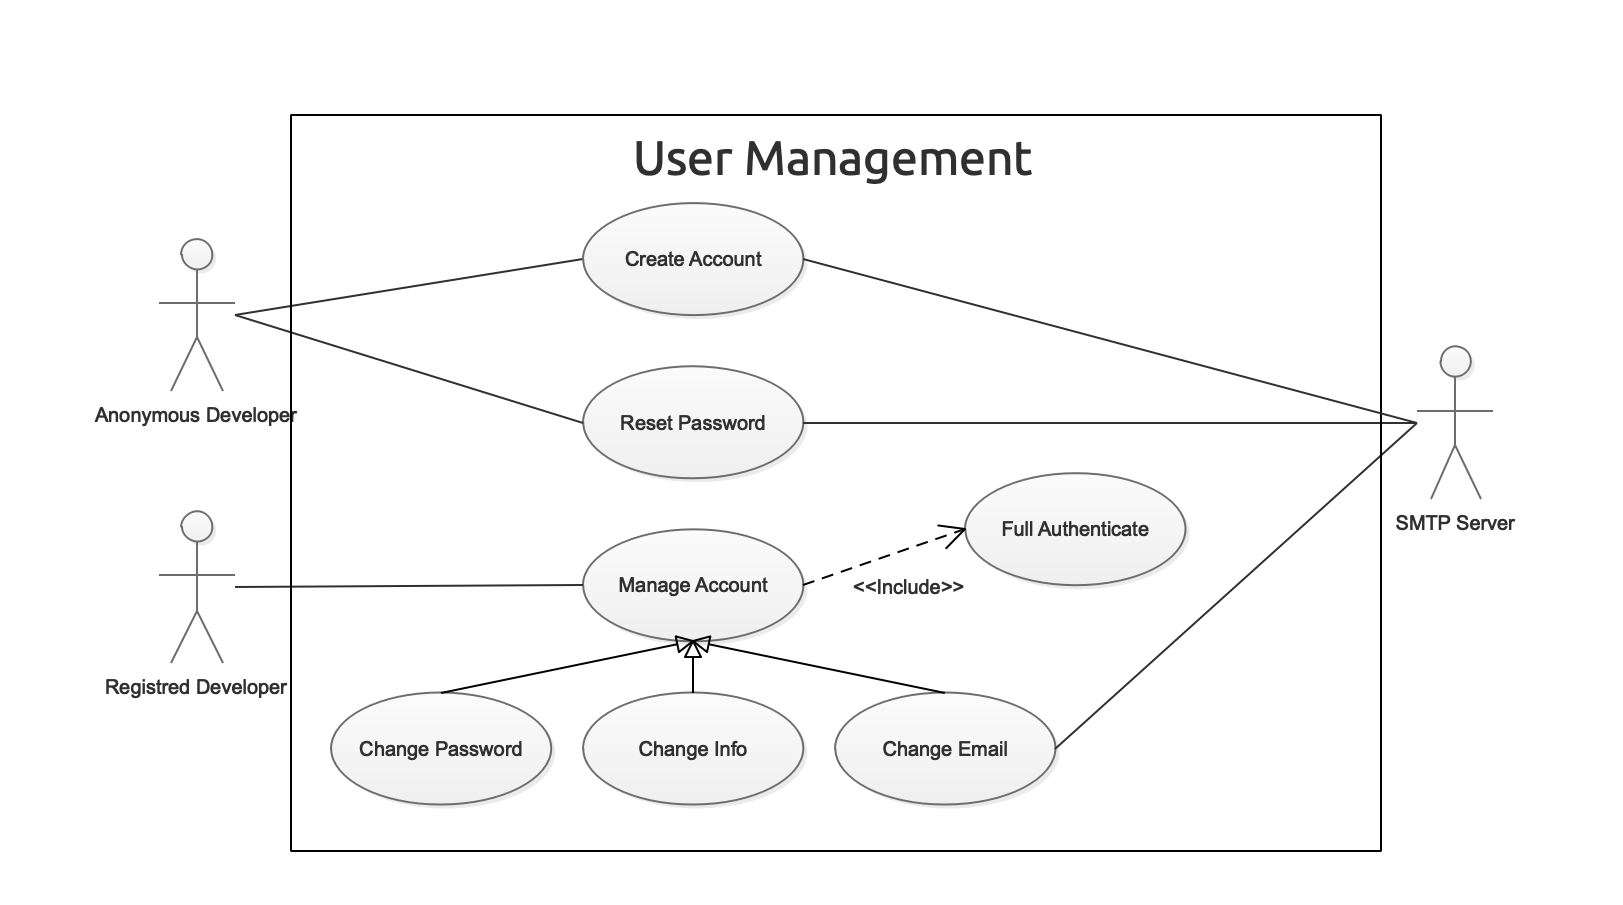
\includegraphics[scale=0.3]{userusecase.png}
\caption{User management use case diagram}
\label{usermanagementusecase}
\end{figure}


\subsection{App management use case}
For every integration, the developer should create an integration app.
The app is linked to a Flouci wallet, and it contains two keys public and private.
The keys are used in the process of integrating the app on e-commerce websites.


The figure \ref{appmanagementusecase} shows the use case diagram, and the table \ref{apptable} is a textual description of the main use case "create app".
\begin{figure}[H]\centering
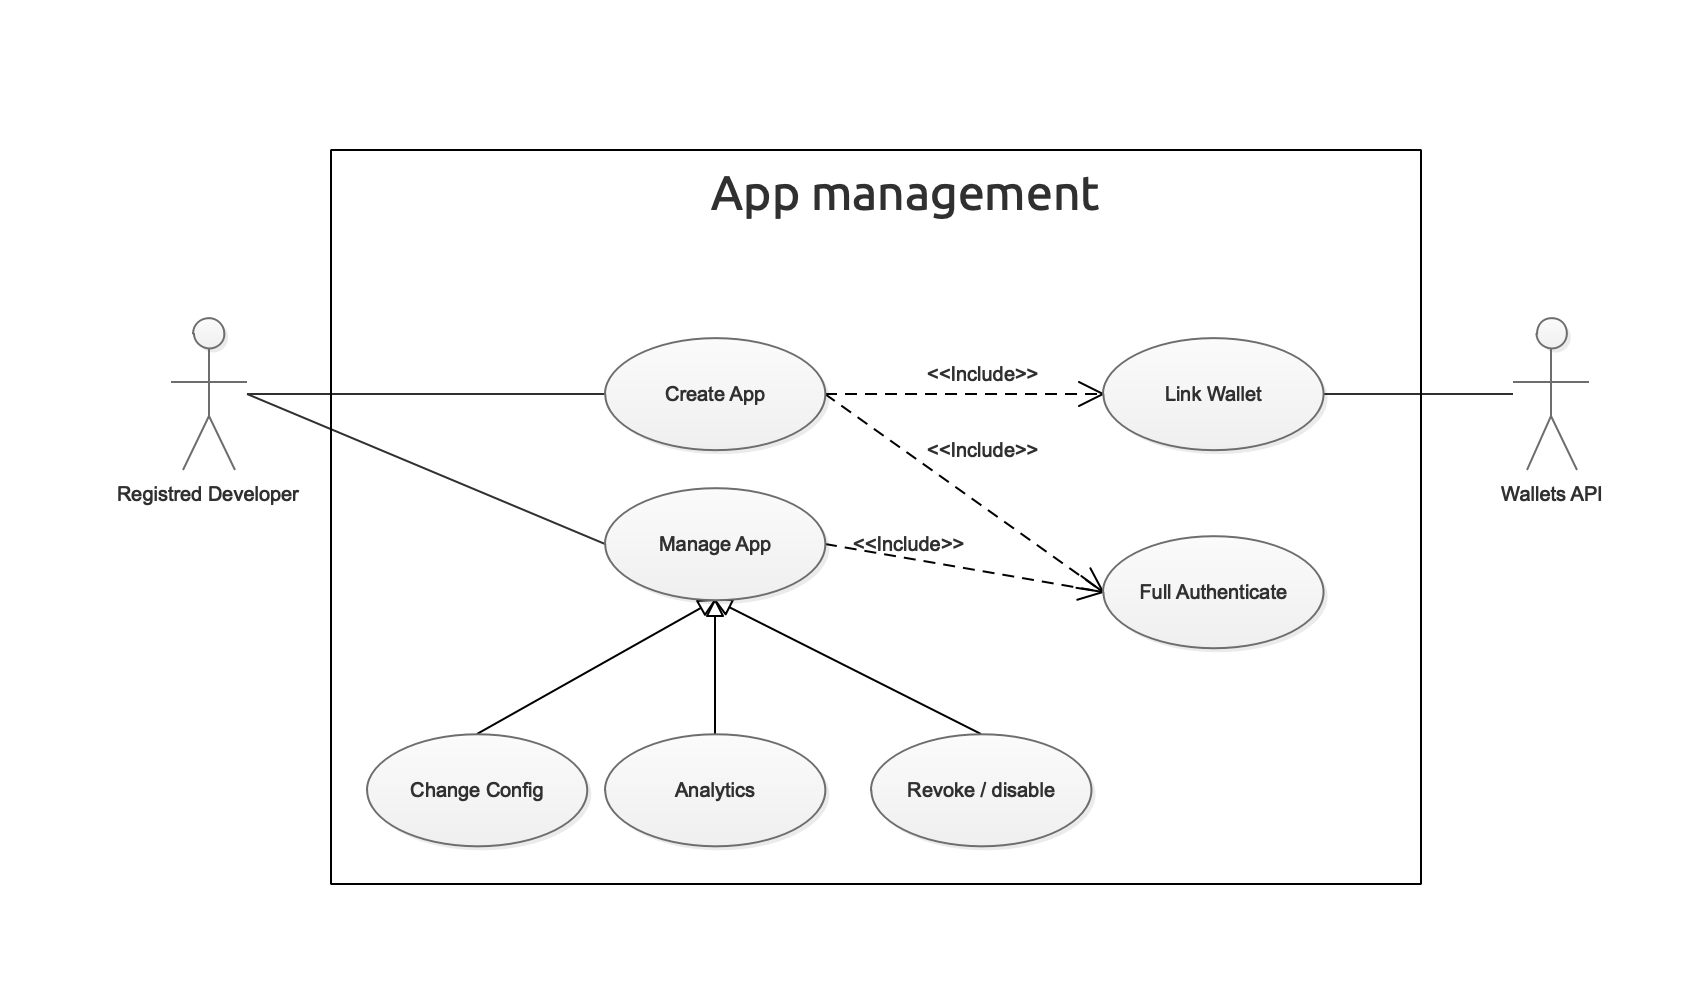
\includegraphics[scale=0.3]{appusecase.png}
\caption{App management use case diagram}
\label{appmanagementusecase}
\end{figure}

\begin{table}[H]
\centering
\caption{Text description of the create app use case}
\begin{tabularx}{\linewidth}{|c|X|}
\hline
Title & create app.  \\ \hline
Summary & The user creates an integration app to use it on his e-commerce website. \\ \hline
Actors & Registered developer. \\ \hline
Precondition & The user visits the new app page. \\ \hline
Nominal Scenario & \begin{enumerate}
 \item The user enters the app name, description and a phone number linked to a Flouci wallet. 
 \item The user gets an OTP on his phone number.
 \item The user enters the OTP to activate the app.
 \item The user is redirected to the newly created app page.
 \end{enumerate}
 \\ \hline
Sc�nario alternatifs & \begin{itemize}
	\item A1 If the app name is already used, the user should change the name.
	\item A2 If the phone number is not linked to a business wallet the user is asked to verify the number.
	\item A3 If the OTP is never received the user can ask to resend OTP.
	\item A3 If the user enters a wrong OTP he is asked to retry with a limit of three times.
\end{itemize} \\ \hline
Exception Scenario & If the user exceeds the maximum number of apps, he cannot create a new app. \\ \hline
Post-condition & The user is redirected to the app page. \\ \hline
\end{tabularx}
\label{apptable}
\end{table}

\section{Platform Design}
Before diving into writing the code, we started by modeling the platform using Adobe XD. This was very helpful for us since it made it possible to focus on the key features we want to have.

The Figure \ref{developersPlatform} represents the Developers API platform model we ended up with. It offers the same user experience of the other Kaoun products including Flouci.

\begin{figure}[H]\centering
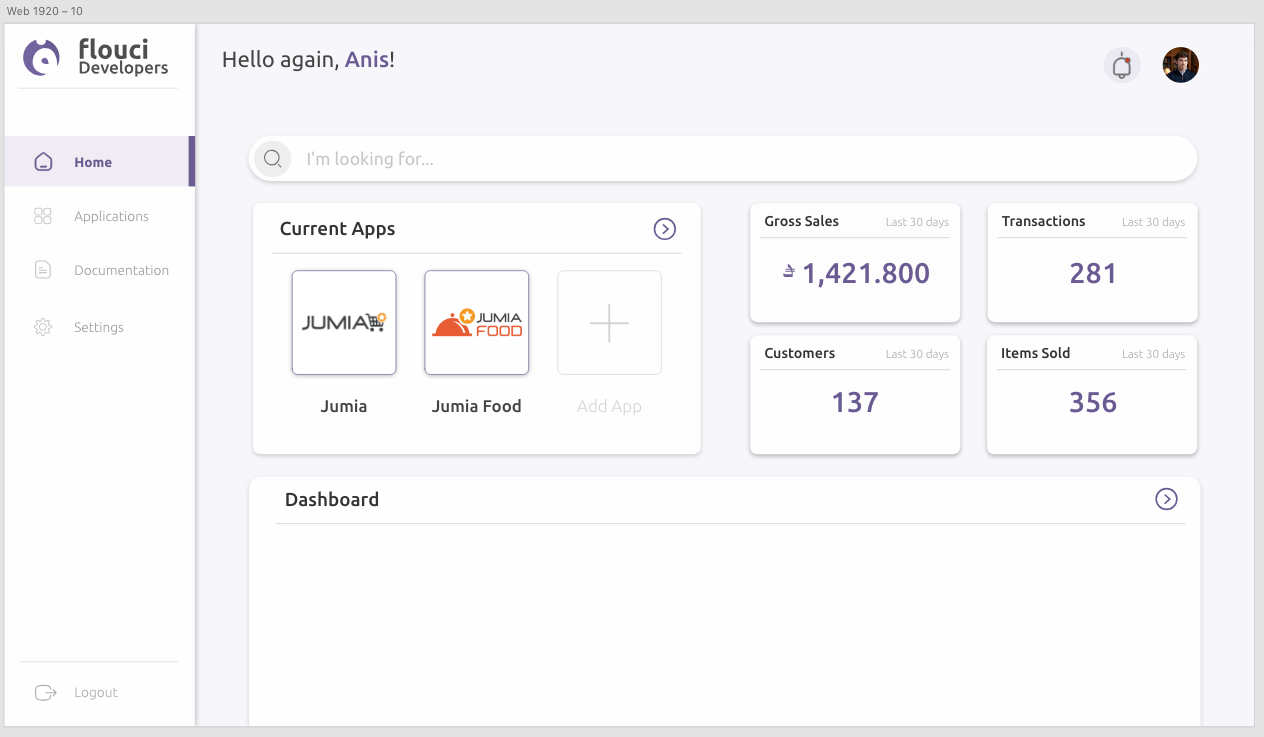
\includegraphics[scale=0.4]{web_screen}
\caption{Developers platform mock-up}
\label{developersPlatform}
\end{figure}

\section{User Management}
In this section we will explain our user management strategy, the mechanism of creating the account and the different authorities used. we also present how to recover a lost account.
\subsection{Authorities}
In our project we used four different authorities to manage access to different parts of the app:
\begin{itemize}
	\item \textbf{System}: who is mainly used by our audit logs, when something is done automatically
	\item \textbf{AnonymousUser:} who is given to anonymous users when they do an action
	\item \textbf{Developer}: who is a normal user with 'ROLE\_DEVELOPER' authorization it gives access to managing apps.
	\item  \textbf{Admin}: who is an admin user with 'ROLE\_DEVELOPER' and 'ROLE\_ADMIN' authorizations, he can manage users.
\end{itemize}

\subsection{Registration}
The registration process is very simple. we only require basic info and a valid email address to open an account. All created accounts have a "DEVELOPER" authorities which basically give them access to restricted functionalities. 

We only activate the user account after the email confirmation. The activation email contains a link with a key saved in the database. Accessing the link will activate the account.

The figure \ref{fig:register} is a sequence diagram that presents all the step needs to create a new account.

\begin{figure}[H]\centering
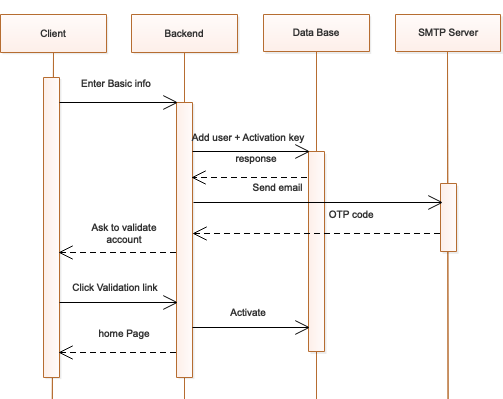
\includegraphics[scale=0.8]{Register_user_sequence_diagram.png}
\caption{User Registration Sequence diagram}
\label{fig:register}
\end{figure}



\subsection{Recover Account}
In case the user forgets his password, he can simply reset it by email. we attach a key to the request and we send the URL with the key to the email. The link with the key takes the user to a page where he can change a new password. After that our backend check the reset key and apply the changes.

\section{App Management}
In our project each e-commerce website is linked to an app to be able to accept Flouci as a payment method.
In this section we will explain key functionalities of the app.
\subsection{App Creation}
Every app is linked to a Flouci Merchant account. Besides the basic information, the developer should enter a phone number to identify the Flouci account then confirm it with the OTP key he gets by SMS.

After finishing creating the app, the developer will obtain two tokens.

The figure \ref{fig:appcreate} shows the whole process in details.
\begin{figure}[H]\centering
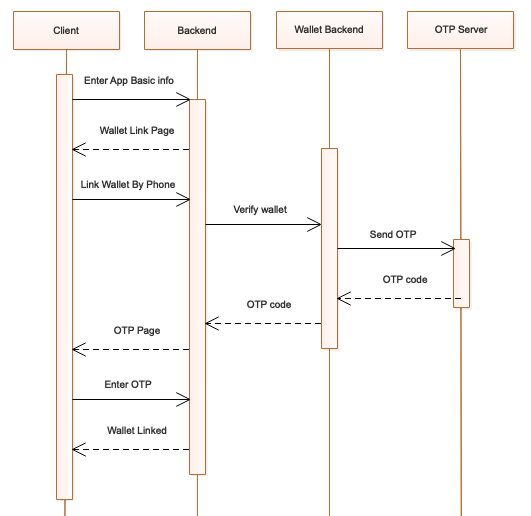
\includegraphics[width=\textwidth,height=12cm]{Create_App_Sequence_Diagram.png}
\caption{App creation Sequence diagram}
\label{fig:appcreate}
\end{figure}
\subsection{App Revoke}
Since the app have two main tokens (public and private), we offer the possibility to revoke an app simply by changing its public token. Changing the token will result in obsoleting all current integration of the app since they all will be using a public token that doesn't resolve our app.

\subsection{App Metrics}
After the integration, there is a huge  risk of the developer shifting a way of the platform. We decided to gather metrics for the user to be able to bring him back to the platform.
Each app have two main metrics.
\begin{itemize}
	\item \textbf{Transactions:} the number of orders made.
	\item \textbf{Gross sales:} the total amount of all orders.
\end{itemize}
We also save the metrics per day with a cron job, so we can easily create charts to monitor sales.

\subsection{Orders}
With every online payment, we attach the app id to the payment payload. This information will help us get the list of orders for each app.
We can then display all orders made, add filtering and even add a button to reimburse orders.

\section{Data schema}
Our database modal can be divided into three big sections of the projects. We have tables managing the user data, Tables managing the app data and others independent tables handling auditing events. Also, we made the modal in a way that the user can have from 0 to N apps and an app can only be linked to one user.
The database schema is presented in the figure \ref{fig:database}
\begin{figure}[H]\centering
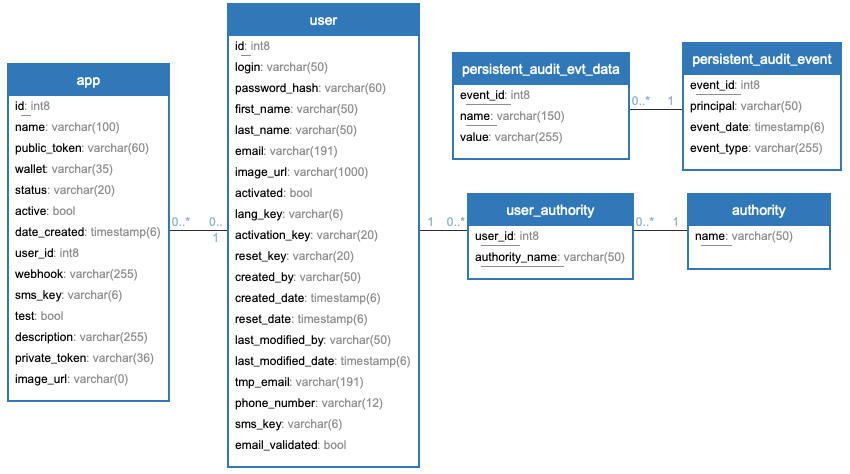
\includegraphics[width=\textwidth,keepaspectratio]{db.png}
\caption{Database modal}
\label{fig:database}
\end{figure}

\section*{Conclusion}
In this section, we implemented the first steps the user should do in order to integrate Flouci. After creating an account and an app, The two tokens provided will be the only missing piece to integrate Flouci payment method.

In the next section, we will implement the checkout API which can be integrated into any e-commerce website.
%==============================================================================
\end{spacing}


\setcounter{chapter}{4}
\chapter{Sprint 3: Checkout Integration}
\minitoc %insert la minitoc
\graphicspath{{Chapter5/figures/}}

%\DoPToC
%==============================================================================
\pagestyle{fancy}
\fancyhf{}
\fancyhead[R]{\bfseries\rightmark}
\fancyfoot[R]{\thepage}
\renewcommand{\headrulewidth}{0.5pt}
\renewcommand{\footrulewidth}{0pt}
\renewcommand{\chaptermark}[1]{\markboth{\MakeUppercase{\chaptername~\thechapter. #1 }}{}}
\renewcommand{\sectionmark}[1]{\markright{\thechapter.\thesection~ #1}}


\begin{spacing}{1.2}

\section*{Introduction}
In this section, we will implement the tools needed for developers to be able to integrate Flouci in their websites. 

In order to make it portable in any existing e-commerce, we decided to implement it in pure javascript.
\section{Front end Integration}
In this section, we will implement the front end payment plugin that can can be integrated in any HTML code.
\subsection{User experience}
In the online payment, we faced a small issue regarding the payment experience, because the process is different from the mobile version. The online payments needs the developer to accept them.
So we decided to create the same QR code experience in mobile and only add a step to enter a six digits code in the browser.

The figure \ref{fig:onlinepay} shows the payment form of the developer API.
\begin{figure}[H]\centering
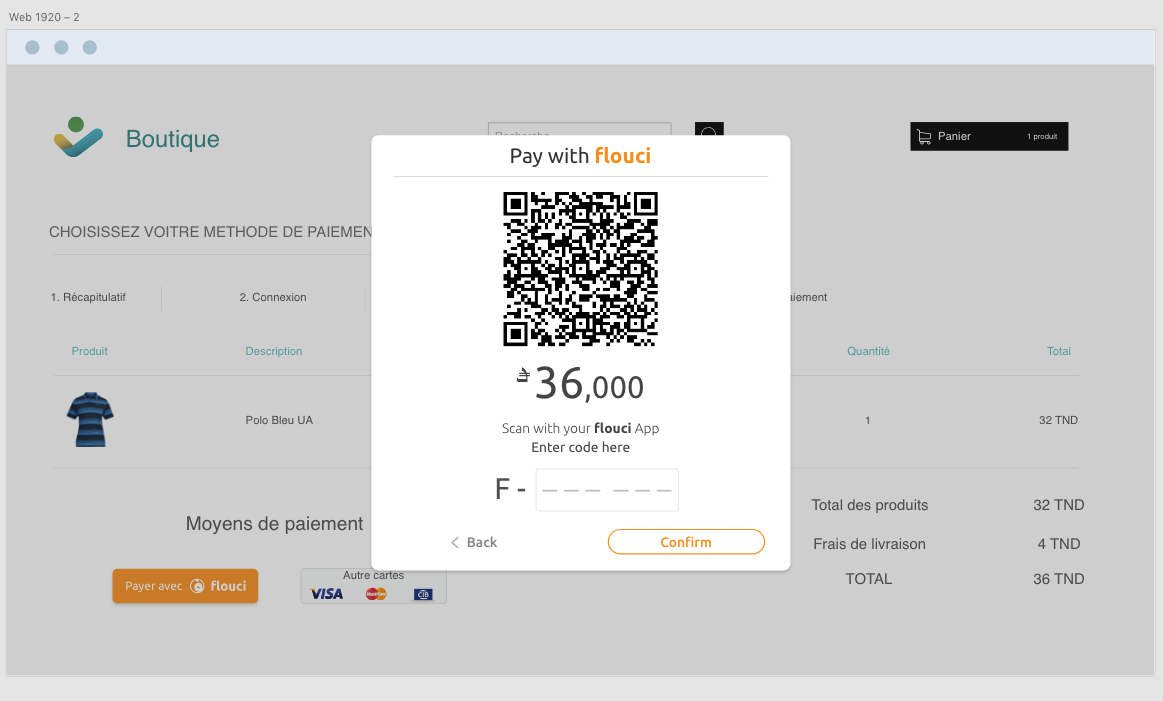
\includegraphics[width= \textwidth, keepaspectratio ]{Checkout_screen.png}
\caption{Flouci payment Form}
\label{fig:onlinepay}
\end{figure}

\subsection{Implementation}
To create our front-end form and make it easy to integrate, we created a web-pack project that bundles next generation javascript and CSS into one single javascript file.
The code contains the payment form and an API validation call to the payment API.
If the six-digit code entered by the user is correct, the script returns the code to the form submit action.
\subsection{Building the script file}
Our front-end integration is basically a web script capable of delivering three main objectives:
\begin{itemize}
	\item \textbf{Payment Button:} The payment button should have a distinct and recognizable style across all e-commerce websites.
	\item \textbf{Payment Form:} The payment form goal is to encode the app public key, amount and other optional fields into one single QR code readable by our Flouci App.
	\item \textbf{Validation API:} After scanning the QR code, the script should be able to validate the pre-payment with the payments API and give feedback to the e-commerce backend.
\end{itemize}

In order to create this script, we had to use different modules such as a QR code generator. This made it impossible to write everything in vanilla javascript and deliver our project on time. 


The solution we agreed on is to create a webpack project. With webpack, we could use next generation javascript and already existing NPM modules then bundle everything in one script. 

The figure \ref{fig:webpack} shows how webpack can transform a javascript module with dependencies into one static bundle.
\begin{figure}[H]\centering
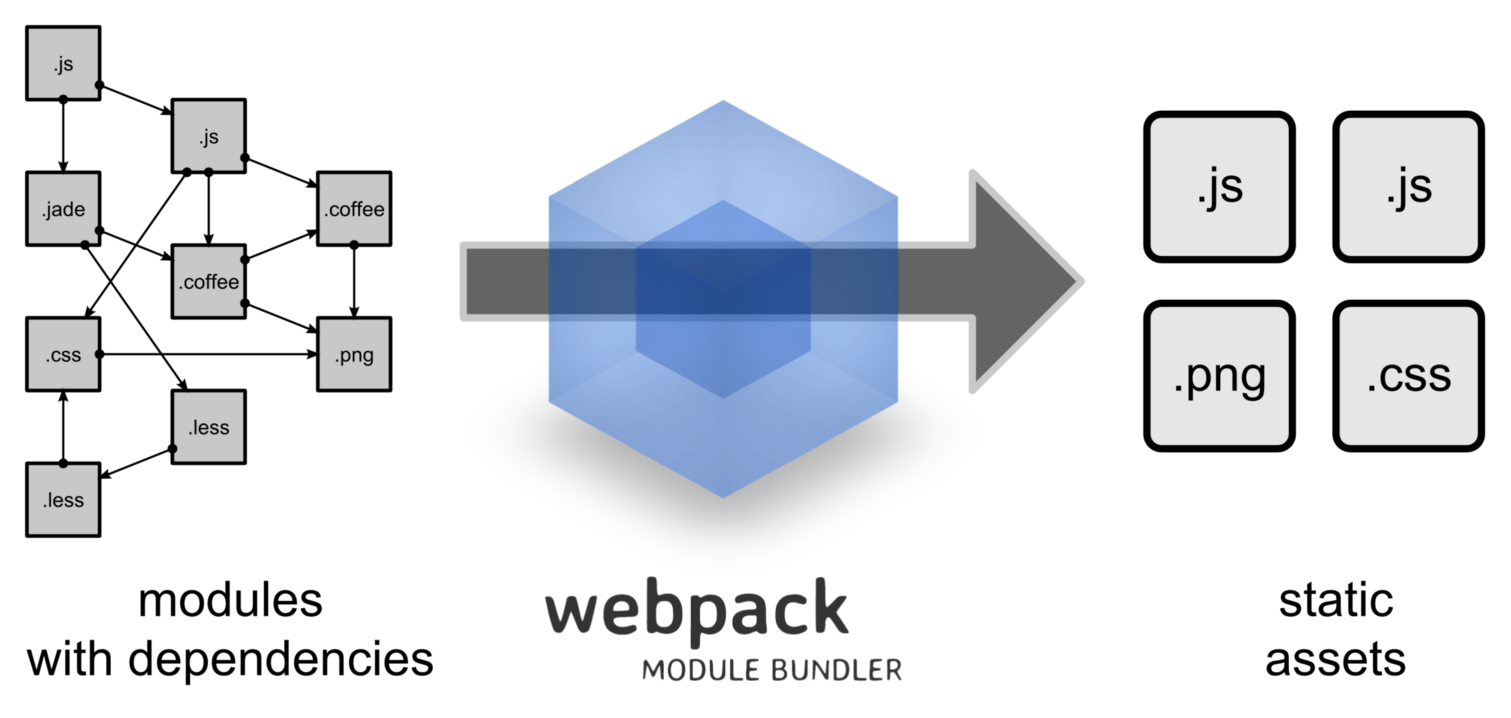
\includegraphics[width=\textwidth, keepaspectratio ]{webpack.png}
\caption{Webpack build process}
\label{fig:webpack}
\end{figure}

\subsection{Design patterns}
In order to implement our solution, we faced a lot of design problems. Luckily such problems were commonly occurring problems in software design. So we studied the known design patterns\cite{designpattern} and we solved our issues with these design patterns:
\begin{itemize}
	\item \textbf{Creational design patterns\cite{designpattern}:} The QR code contains different fields so we followed the Builder design pattern to create it.
	\item \textbf{Structural design patterns\cite{designpattern}:} Our form hide different components and complex behavior so we implemented a Facade design pattern to deliver a single class that 
	 represents the entire subsystem.
	 \item \textbf{Behavioral design patterns\cite{designpattern}:} The process of payments include different steps, that's why we implemented a  Chain of responsibility design pattern to pass the payment request between our three main objects.
\end{itemize}
\subsection{Integration}
After hosting the javascript file we can easily add the form to our project. The form will only require the public app key  and the amount.
The HTML code is listed in \ref{code:html}.
\begin{lstlisting}[rulecolor=\color{white}]
\end{lstlisting}
\begin{lstlisting}[label=code:html,caption=Flouci Integration Java,language=xml]
 <form id="myform" action="/handle_payment" method="post">
    <script
            src="https://developersdev.flouci.com/static/main.js"
            data-key="f6b5d0a5-e559-4acb-bcbb-a9e6ec9d788d"
            data-amount="2700000"
            data-name="Flouci Checkout"
            data-description="Flouci Data"

    </script>
  </form>
\end{lstlisting}


\section{Back end Integration}
After the user inputs the six digits code into the form, the form checks the validity of the payment and return a special key to the backend ( the action function inputed by the developer)

The developer then is only required to call an endpoint to accept the payment and then redirects the user to an other page depending on the payment result. 

In the figure \ref{fig:flask} we show the code of a simple flask server with a Flouci integration that works with the HTML code listed in \ref{code:html}.
\begin{figure}[H]\centering
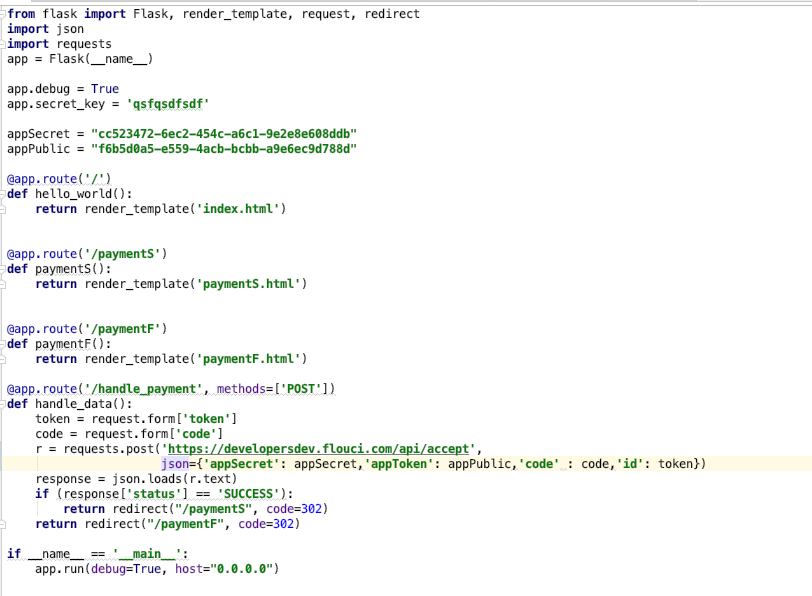
\includegraphics[width=\textwidth,height=12cm]{flask.png}
\caption{Flouci payment Backend Integration}
\label{fig:flask}
\end{figure}
\section{Payment process}
To summarize the payment process, we created a sequence diagram prsented in the figure \ref{fig:FPSD} that contains all the interactions needed to process a payment.
\begin{figure}[H]\centering
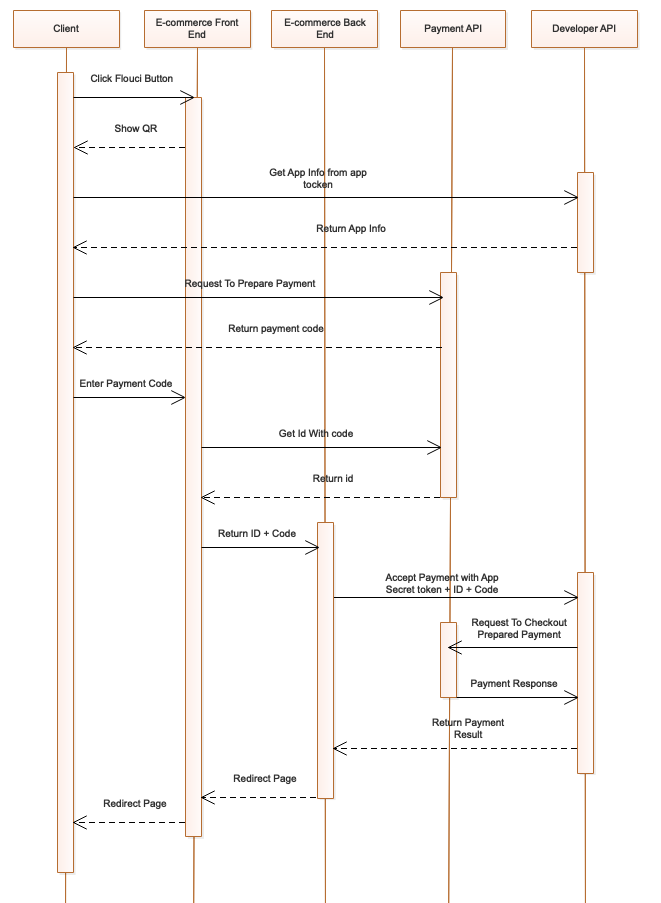
\includegraphics[width=\textwidth,height=18cm]{Payment_Sequence_Diagram.png}
\caption{Flouci payment Sequence Diagram}
\label{fig:FPSD}
\end{figure}
In order to make a payment, the user should click the payment button and scan the QR code. The mobile app then gets the app info from the developer API and verify its validity. If the app is valid the mobile phone call the payment API to prepare the payment, this will return a key. The user inputs the key into the form and then the form will call the payment API to verify it and get an extra id to return it to the developer backend. Finally the developer should call the developer api and send his app secret, the key and the id returned by the form, the developer api calls the payment api to execute the payment and return the result to the developer.
\section*{Conclusion}
In this chapter we implemented the checkout API, which serve as an integration module that can be integrated in any web based project.

In the implementation of our solution we had to made it the simplest integration possible and the most portable one. And we made as easy as implementing a simple REST call. 

With the checkout integration module, we finally have all the pieces needed in the Flouci online payment process. We now have a fully functional project.

\end{spacing}



\backmatter
\pagestyle{fancy}
\fancyhf{}
\renewcommand{\chaptermark}[1]{\markboth{Conclusion Generale et Perspectives}{}}
\fancyhead[R]{Conclusion Generale et Perspectives}
\fancyfoot[R]{\thepage}
\renewcommand{\headrulewidth}{0.5pt}
\renewcommand{\footrulewidth}{0pt}
\chapter{General Conclusion and Perspectives }
%==============================================================================
\pagestyle{fancy}
\fancyhf{}
\fancyhead[R]{\bfseries\rightmark}
\fancyfoot[R]{\thepage}
\renewcommand{\headrulewidth}{0.5pt}
\renewcommand{\footrulewidth}{0pt}
\renewcommand{\chaptermark}[1]{\markboth{\MakeUppercase{\chaptername~\thechapter. #1 }}{}}
\renewcommand{\sectionmark}[1]{\markright{\thechapter.\thesection~ #1}}

\begin{spacing}{1.2}
%==============================================================================
During a period of four months, we had to design and implement our challenging project. We needed to expand the Flouci ecosystem and add the ability to perform online integrations.
The project had to involve a lot of pieces, A platform that allows developers to manage their integration, A module that could be integrated into e-commerce websites, As well as the existing API's of The Flouci ecosystem including the payment API and the Wallets API.   

We started our work by setting up a modern software development discipline. We followed the Kanban methodology and created our project board from day one. We also defined a DevOps pipeline that involves different steps from testing to packaging and deploying. And we followed a strict TDD to ensure that we have a good testing coverage. 

Only after making sure that we can write code in the best quality possible and making the development experience as modern as we could that we started implementing our core functionalities. 

First, we started implementing the developer's platform, We challenged ourselves to build the front end in React, Since the company was shifting all its products to react and that's when we knew that in order to finish our product we needed to be adapt and learn anything.

After finishing our platform, we dived into the next sprint and started developing the integration module. The hardest part of the project was to make the module as portable as possible, and we had to make it in pure javascript.  

In the end, we delivered a platform to create integration apps, as well as a simple module that could use those apps to add the Flouci payment method on any website. It only takes the knowledge of performing a REST call to complete the integration.

From this state, our project could evolve and add more functionalities:
\begin{itemize}
	\item \textbf{Plateform:} We could add more customization to our integration app and allow developers to add their users and items. After that we can add more metrics relevant to items or users like most sold items, or most active customers.
	\item \textbf{Checkout module:} we can add the possibility to pay with the Flouci login credentials, and also we can make a button that redirects to the app on mobile devices to perform payments without having to scan any QR codes.
\end{itemize} 

%==============================================================================
\end{spacing}

\bibliographystyle{Biblio/unsrt_modif}
\singlespacing
\renewcommand{\bibname}{Bibliographique}

\bibliography{Biblio/aesm_edspia}

\onehalfspacing

\appendix

\end{document}
